% =====================================================================
%  Silent order corruption in per-sample evaluation artefacts
%  Elsevier CAS single-column manuscript (cas-sc).
%
%  NO NUMBER IS TYPED IN THIS FILE. Every quantitative claim expands a
%  macro from paper/numbers.tex, which is generated by
%      python tools/paper_assets.py numbers
%  from the artefacts in artifacts/. Tables and figures are generated by
%      python tools/paper_assets.py tables
%      python tools/paper_assets.py figs
%  and tools/verify_paper_numbers.py re-derives every macro from the
%  artefacts and fails the build on any mismatch.
%
%  Build:  pdflatex main && bibtex main && pdflatex main && pdflatex main
% =====================================================================
\documentclass[a4paper,fleqn]{cas-sc}

\usepackage[numbers]{natbib}
\usepackage{amsmath,amssymb}
\usepackage{booktabs}
\usepackage{graphicx}
\usepackage{listings}
\usepackage{xcolor}

\newtheorem{proposition}{Proposition}
\newtheorem{corollary}[proposition]{Corollary}
\newtheorem{definition}[proposition]{Definition}
\newproof{pf}{Proof}

\setlength{\tabcolsep}{4pt}

% Shrink a table to the text width *only* when it is genuinely too wide;
% a bare \resizebox would also magnify narrow tables.
\newcommand{\fitwidth}[1]{%
  \resizebox{\ifdim\width>\linewidth \linewidth\else \width\fi}{!}{#1}}

\definecolor{codekw}{RGB}{20,80,140}
\definecolor{codecm}{RGB}{110,110,110}
\definecolor{codestr}{RGB}{140,60,40}
\lstdefinestyle{py}{
  language=Python, basicstyle=\ttfamily\footnotesize,
  keywordstyle=\color{codekw}\bfseries, commentstyle=\color{codecm}\itshape,
  stringstyle=\color{codestr}, showstringspaces=false,
  numbers=left, numberstyle=\tiny\color{codecm}, numbersep=6pt,
  frame=single, rulecolor=\color{codecm}, framesep=4pt,
  breaklines=true, columns=fullflexible, keepspaces=true, aboveskip=8pt,
  belowskip=6pt, xleftmargin=14pt,
}
\lstset{style=py}

% Corresponding e-mail address, defined inside a catcode-safe group so that an
% underscore in the local part cannot break the build; edit only this one line.
% \ead detokenises its argument, so the macro must be expanded *before* \ead
% sees it (see \expandafter below).
\begingroup
\catcode`\_=12
\gdef\correspemail{1367489893@qq.com}
\gdef\secondemail{1577027526@qq.com}
\endgroup

% No ORCID is registered for this submission; suppress the empty "ORCID(s):"
% footnote that cas-sc emits unconditionally on the title page.
\AtBeginDocument{\renewcommand{\printorcid}{}}

% All numeric claims live here (generated file).
% Generated by tools/paper_assets.py numbers -- do not edit by hand.
% Every numeric claim in main.tex expands one of these macros.

\newcommand{\NumArms}{4}
\newcommand{\NumBackbones}{3}
\newcommand{\NumBackfillDirs}{356}
\newcommand{\NumBackfillFailures}{0}
\newcommand{\NumBackfillSidecars}{1\,424}
\newcommand{\NumBatAotDisjoint}{2.1}
\newcommand{\NumBatAotStrideOne}{100}
\newcommand{\NumBatCatDisjoint}{100}
\newcommand{\NumBatCatStrideOne}{98.9}
\newcommand{\NumBatCorruptAotMax}{66.7}
\newcommand{\NumBatCorruptAotPct}{6}
\newcommand{\NumBatCorruptCatMax}{100}
\newcommand{\NumBatCorruptCatPct}{3.7}
\newcommand{\NumBatDisjointRows}{16}
\newcommand{\NumBatGroups}{95}
\newcommand{\NumBatNDisjoint}{60}
\newcommand{\NumBatRows}{758}
\newcommand{\NumBatStrideDisjoint}{192}
\newcommand{\NumBlocks}{56}
\newcommand{\NumCalibFprNormal}{9.17}
\newcommand{\NumCalibFprPerm}{7.5}
\newcommand{\NumCalibMaxAbsDiff}{0.0262}
\newcommand{\NumCalibSeq}{120}
\newcommand{\NumCatAnalyticErrMax}{0.0215}
\newcommand{\NumCatAnalyticErrMedian}{0.0042}
\newcommand{\NumCatAnalyticNaiveErrMax}{0.2051}
\newcommand{\NumCatAnalyticNaiveErrMedian}{0.1167}
\newcommand{\NumCatAnalyticPairs}{6}
\newcommand{\NumCatAnalyticRows}{24}
\newcommand{\NumCatBlocks}{96}
\newcommand{\NumCatCertCleanPct}{99}
\newcommand{\NumCatCertCorruptPct}{4.17}
\newcommand{\NumCatCondAllSharedCert}{24}
\newcommand{\NumCatCondAllSharedRho}{0.9509}
\newcommand{\NumCatCondGroups}{24}
\newcommand{\NumCatCondIndependentCert}{0}
\newcommand{\NumCatCondIndependentRho}{-0.0023}
\newcommand{\NumCatCondIntactCert}{24}
\newcommand{\NumCatCondIntactRho}{0.9509}
\newcommand{\NumCatCondRows}{144}
\newcommand{\NumCatCondSharedKThreeCert}{24}
\newcommand{\NumCatCondSharedKThreeRho}{0.4827}
\newcommand{\NumCatCondSharedKTwoCert}{24}
\newcommand{\NumCatCondSharedKTwoRho}{0.1579}
\newcommand{\NumCatCondTwoPairsCert}{24}
\newcommand{\NumCatCondTwoPairsRho}{0.3199}
\newcommand{\NumCatMinN}{38}
\newcommand{\NumCatMissGroups}{1}
\newcommand{\NumCatMissMaxN}{41}
\newcommand{\NumCatPairRhoMedian}{0.9507}
\newcommand{\NumCatPairs}{492}
\newcommand{\NumCatRhoMedianClean}{0.9371}
\newcommand{\NumCatRhoMedianCorrupt}{-0.002}
\newcommand{\NumCatRhoMinClean}{-0.192}
\newcommand{\NumCatSdRatioCorrectedMedian}{1.0039}
\newcommand{\NumCatSdRatioNaiveMedian}{0.4098}
\newcommand{\NumCatSdRatioNaiveTheory}{0.4082}
\newcommand{\NumCertTwelveMissMaxN}{50}
\newcommand{\NumCertTwelveMissSeq}{18}
\newcommand{\NumCleanCertAlphaSix}{100}
\newcommand{\NumCleanCertAlphaThree}{100}
\newcommand{\NumCleanCertAlphaTwelve}{97.5}
\newcommand{\NumCleanCertPct}{100}
\newcommand{\NumContractAdversarialTests}{33}
\newcommand{\NumContractDetected}{20}
\newcommand{\NumContractFaults}{25}
\newcommand{\NumContractRepoTests}{99}
\newcommand{\NumContractUndetected}{5}
\newcommand{\NumCorruptCertAlphaSix}{0}
\newcommand{\NumCorruptCertAlphaThree}{0.14}
\newcommand{\NumCorruptCertAlphaTwelve}{0}
\newcommand{\NumCorruptCertPct}{6.18}
\newcommand{\NumDatasets}{7}
\newcommand{\NumDepBlockLenCappedCells}{46}
\newcommand{\NumDepBlockLenMedian}{212}
\newcommand{\NumDepBlockSigDatasetCiHigh}{60.67}
\newcommand{\NumDepBlockSigDatasetCiLow}{8.43}
\newcommand{\NumDepBlockSigPct}{34.27}
\newcommand{\NumDepBlockSigSampleSetCiHigh}{57.93}
\newcommand{\NumDepBlockSigSampleSetCiLow}{10.05}
\newcommand{\NumDepBootCiExclDatasetCiHigh}{53.09}
\newcommand{\NumDepBootCiExclDatasetCiLow}{9.16}
\newcommand{\NumDepBootCiExclPct}{32.87}
\newcommand{\NumDepBootCiExclSampleSetCiHigh}{55.15}
\newcommand{\NumDepBootCiExclSampleSetCiLow}{11.14}
\newcommand{\NumDepCells}{356}
\newcommand{\NumDepClusterBoot}{4\,000}
\newcommand{\NumDepClusterDatasets}{7}
\newcommand{\NumDepClusterSampleSets}{28}
\newcommand{\NumDepDatasets}{7}
\newcommand{\NumDepDefectMinusControlDatasetCiHigh}{0.000465}
\newcommand{\NumDepDefectMinusControlDatasetCiLow}{-0.001907}
\newcommand{\NumDepDefectMinusControlMedian}{-0.000526}
\newcommand{\NumDepDefectMinusControlSampleSetCiHigh}{0.000868}
\newcommand{\NumDepDefectMinusControlSampleSetCiLow}{-0.002811}
\newcommand{\NumDepIidSigDatasetCiHigh}{97.98}
\newcommand{\NumDepIidSigDatasetCiLow}{73.19}
\newcommand{\NumDepIidSigPct}{89.33}
\newcommand{\NumDepIidSigSampleSetCiHigh}{95.64}
\newcommand{\NumDepIidSigSampleSetCiLow}{79.88}
\newcommand{\NumDepMinHoldoutWindows}{200}
\newcommand{\NumDepNBoot}{2\,000}
\newcommand{\NumDepNPerm}{2\,000}
\newcommand{\NumDepRhoDatasetCiHigh}{0.2812}
\newcommand{\NumDepRhoDatasetCiLow}{0.0871}
\newcommand{\NumDepRhoIqr}{0.2224}
\newcommand{\NumDepRhoMax}{0.7862}
\newcommand{\NumDepRhoMedian}{0.2192}
\newcommand{\NumDepRhoMin}{-0.7341}
\newcommand{\NumDepRhoQOne}{0.07}
\newcommand{\NumDepRhoQThree}{0.2925}
\newcommand{\NumDepRhoSampleSetCiHigh}{0.2731}
\newcommand{\NumDepRhoSampleSetCiLow}{0.1049}
\newcommand{\NumDepSampleSets}{56}
\newcommand{\NumDepSampleSetsVal}{28}
\newcommand{\NumDepSequences}{712}
\newcommand{\NumDistinctWindows}{287\,496}
\newcommand{\NumEqDrawRhoAbsDiffMax}{0.0097}
\newcommand{\NumEqDrawRhoCertPct}{100}
\newcommand{\NumEqDrawRhoCiHigh}{0.0024}
\newcommand{\NumEqDrawRhoCiLow}{-0.0023}
\newcommand{\NumEqDrawRhoMeanDiff}{0.0001}
\newcommand{\NumEqDrawRhoP}{\ensuremath{3.11\times 10^{-80}}}
\newcommand{\NumEqDrawRhoSinglePMax}{\ensuremath{2.77\times 10^{-8}}}
\newcommand{\NumEqDrawRhoSinglePMedian}{\ensuremath{4.89\times 10^{-13}}}
\newcommand{\NumEqDrawTransferAbsDiffMax}{0.0125}
\newcommand{\NumEqDrawTransferCertPct}{100}
\newcommand{\NumEqDrawTransferCiHigh}{0.0102}
\newcommand{\NumEqDrawTransferCiLow}{-0.0022}
\newcommand{\NumEqDrawTransferMeanDiff}{0.004}
\newcommand{\NumEqDrawTransferP}{\ensuremath{2.24\times 10^{-15}}}
\newcommand{\NumEqDrawTransferSinglePMax}{0.0215}
\newcommand{\NumEqDrawTransferSinglePMedian}{0.0125}
\newcommand{\NumEqDraws}{8}
\newcommand{\NumGpuHours}{21.3}
\newcommand{\NumLabelBestFixedShareDefectPct}{33.1}
\newcommand{\NumLabelBestFixedShareIndexPct}{45.7}
\newcommand{\NumLabelBlocks}{96}
\newcommand{\NumLabelEntropyDefect}{1.822}
\newcommand{\NumLabelEntropyIndex}{1.653}
\newcommand{\NumLabelEntropyMax}{2}
\newcommand{\NumLabelModalDefectPct}{33.3}
\newcommand{\NumLabelModalIndexPct}{46.1}
\newcommand{\NumMaskChecked}{96}
\newcommand{\NumMaskLengthPct}{100}
\newcommand{\NumMaskMaxRelMeanDiff}{0}
\newcommand{\NumMaskMultisetPct}{100}
\newcommand{\NumObsAotFlagArms}{87}
\newcommand{\NumObsAotFlagPct}{90.63}
\newcommand{\NumObsAotMissArms}{9}
\newcommand{\NumObsAotMissGroups}{6}
\newcommand{\NumObsAotPMin}{0.00412}
\newcommand{\NumObsCatCertGroups}{22}
\newcommand{\NumObsCatCertIntactGroups}{24}
\newcommand{\NumObsCatCertIntactPct}{100}
\newcommand{\NumObsCatCertPct}{91.67}
\newcommand{\NumObsCatRhoIntactMedian}{0.9509}
\newcommand{\NumObsCatRhoMedian}{0.4189}
\newcommand{\NumObsPairsIdenticalNone}{2}
\newcommand{\NumObsPairsIdenticalOne}{7}
\newcommand{\NumObsPairsIdenticalSix}{2}
\newcommand{\NumObsPairsIdenticalThree}{11}
\newcommand{\NumObsPairsIdenticalTwo}{2}
\newcommand{\NumObsPermAllDistinct}{2}
\newcommand{\NumObsPermAllIdentical}{2}
\newcommand{\NumObsPermArms}{96}
\newcommand{\NumObsPermConsistentGroups}{24}
\newcommand{\NumObsPermGroups}{24}
\newcommand{\NumObsPermNonIdentityArms}{96}
\newcommand{\NumObsPermPairs}{144}
\newcommand{\NumObsPermPartialShared}{20}
\newcommand{\NumObsSpearmanMax}{1}
\newcommand{\NumObsSpearmanMedian}{0.4874}
\newcommand{\NumObsSpearmanMin}{0.0001}
\newcommand{\NumObservedCertPct}{9.38}
\newcommand{\NumObservedRMedian}{-0.0003}
\newcommand{\NumObservedSeq}{96}
\newcommand{\NumPurgeBucketCells}{20}
\newcommand{\NumPurgeBucketPredLen}{720}
\newcommand{\NumPurgeBucketSeqLen}{96}
\newcommand{\NumPurgeCells}{356}
\newcommand{\NumPurgeDisjointEligible}{310}
\newcommand{\NumPurgeDisjointGap}{817}
\newcommand{\NumPurgeDisjointIneligible}{46}
\newcommand{\NumPurgeDisjointOrigins}{408}
\newcommand{\NumPurgeDisjointRequiredGap}{816}
\newcommand{\NumPurgeDisjointSharedTarget}{0}
\newcommand{\NumPurgeDisjointSharedTime}{0}
\newcommand{\NumPurgeLabelsEligible}{310}
\newcommand{\NumPurgeLabelsGap}{721}
\newcommand{\NumPurgeLabelsIneligible}{46}
\newcommand{\NumPurgeLabelsOrigins}{360}
\newcommand{\NumPurgeLabelsRequiredGap}{720}
\newcommand{\NumPurgeLabelsSharedTarget}{0}
\newcommand{\NumPurgeLabelsSharedTime}{95}
\newcommand{\NumPurgeLegacyGap}{401}
\newcommand{\NumPurgeLegacyLeakCells}{28}
\newcommand{\NumPurgeLegacyOrigins}{200}
\newcommand{\NumPurgeLegacySharedTarget}{319}
\newcommand{\NumPurgeLegacySharedTime}{415}
\newcommand{\NumRMaxCorrupt}{0.4617}
\newcommand{\NumRMedianClean}{0.9975}
\newcommand{\NumRMedianCorrupt}{0.0011}
\newcommand{\NumRMinClean}{0.85}
\newcommand{\NumRhoMinNHundred}{0.2926}
\newcommand{\NumRhoMinNThousand}{0.0925}
\newcommand{\NumRuns}{356}
\newcommand{\NumRunsDet}{260}
\newcommand{\NumRunsShuf}{96}
\newcommand{\NumSampleSets}{56}
\newcommand{\NumSensBlockMax}{512}
\newcommand{\NumSensBlockMaxRate}{100}
\newcommand{\NumSensFlagBlockMax}{0}
\newcommand{\NumSensFlagPartialFull}{95}
\newcommand{\NumSensFlagPartialHalf}{1.67}
\newcommand{\NumSensFlagPartialMildMax}{0}
\newcommand{\NumSensFlagPartialQuarter}{1.67}
\newcommand{\NumSensNBlockRows}{235}
\newcommand{\NumSensNPartialRows}{300}
\newcommand{\NumSensPartialFullRate}{5}
\newcommand{\NumSensPartialMin}{5}
\newcommand{\NumSensPartialMinRate}{100}
\newcommand{\NumSensSeq}{60}
\newcommand{\NumSequences}{712}
\newcommand{\NumTailKurtMax}{14.1}
\newcommand{\NumTailMaxZ}{5.59}
\newcommand{\NumTailNullDraws}{2\,500\,000}
\newcommand{\NumTailPerm}{500\,000}
\newcommand{\NumTailRatioAboveOnePct}{80}
\newcommand{\NumTailRatioAboveOneRows}{20}
\newcommand{\NumTailRatioFive}{2.8}
\newcommand{\NumTailRatioFour}{2.3}
\newcommand{\NumTailRatioMedianFive}{2}
\newcommand{\NumTailRatioMedianFour}{1.72}
\newcommand{\NumTailRatioMedianSix}{2}
\newcommand{\NumTailRatioMedianThree}{1.472}
\newcommand{\NumTailRatioMedianTwo}{1.1642}
\newcommand{\NumTailRatioSix}{10}
\newcommand{\NumTailRatioThree}{1.77}
\newcommand{\NumTailRatioTwo}{1.26}
\newcommand{\NumTailSeq}{5}
\newcommand{\NumTailShortMaxZ}{4.55}
\newcommand{\NumTailShortN}{38}
\newcommand{\NumTaskOneCells}{356}
\newcommand{\NumTaskOneDecileControlMedian}{1}
\newcommand{\NumTaskOneDecileDefectMedian}{0.995}
\newcommand{\NumTaskOneDecileIndexMedian}{1.426}
\newcommand{\NumTaskOneHoldoutControlMedian}{-0.0005}
\newcommand{\NumTaskOneHoldoutDefectMedian}{0}
\newcommand{\NumTaskOneHoldoutIndexMedian}{0.1191}
\newcommand{\NumTaskOneRhoBestControlMedian}{0.0271}
\newcommand{\NumTaskOneRhoBestDefectMedian}{0.0267}
\newcommand{\NumTaskOneRhoBestIndexMedian}{0.2817}
\newcommand{\NumTaskOneRhoControlMean}{-0.0012}
\newcommand{\NumTaskOneRhoControlMedian}{0.0014}
\newcommand{\NumTaskOneRhoDefectMean}{-0.0007}
\newcommand{\NumTaskOneRhoDefectMedian}{-0.0004}
\newcommand{\NumTaskOneRhoIndexMean}{0.1668}
\newcommand{\NumTaskOneRhoIndexMedian}{0.2192}
\newcommand{\NumTaskOneSigControlPct}{5.3}
\newcommand{\NumTaskOneSigDefectPct}{3.9}
\newcommand{\NumTaskOneSigIndexPct}{89.3}
\newcommand{\NumTaskOneTostCiHigh}{0.00604}
\newcommand{\NumTaskOneTostCiLow}{-0.00495}
\newcommand{\NumTaskOneTostClusterCiHigh}{0.00495}
\newcommand{\NumTaskOneTostClusterCiLow}{-0.00286}
\newcommand{\NumTaskOneTostClusterP}{\ensuremath{9.00\times 10^{-7}}}
\newcommand{\NumTaskOneTostClusters}{7}
\newcommand{\NumTaskOneTostMargin}{0.03}
\newcommand{\NumTaskOneTostMeanDiff}{0.00055}
\newcommand{\NumTaskOneTostP}{\ensuremath{4.46\times 10^{-23}}}
\newcommand{\NumTaskOneTransferControlMean}{-0.0053}
\newcommand{\NumTaskOneTransferControlMedian}{-0.0076}
\newcommand{\NumTaskOneTransferDefectMean}{0.0107}
\newcommand{\NumTaskOneTransferDefectMedian}{0.0156}
\newcommand{\NumTaskOneTransferIndexMean}{0.1902}
\newcommand{\NumTaskOneTransferIndexMedian}{0.2275}
\newcommand{\NumTaskOneTransferTostCiHigh}{0.0329}
\newcommand{\NumTaskOneTransferTostCiLow}{-0.001}
\newcommand{\NumTaskOneTransferTostClusterCiHigh}{0.0378}
\newcommand{\NumTaskOneTransferTostClusterCiLow}{0.0029}
\newcommand{\NumTaskOneTransferTostClusterP}{0.106}
\newcommand{\NumTaskOneTransferTostMargin}{0.03}
\newcommand{\NumTaskOneTransferTostMeanDiff}{0.01595}
\newcommand{\NumTaskOneTransferTostN}{324}
\newcommand{\NumTaskOneTransferTostP}{0.0517}
\newcommand{\NumTaskTwoBlocks}{96}
\newcommand{\NumTaskTwoGainControlMean}{-1.222}
\newcommand{\NumTaskTwoGainControlMedian}{-0.287}
\newcommand{\NumTaskTwoGainControlPosPct}{15.6}
\newcommand{\NumTaskTwoGainDefectMean}{-1.809}
\newcommand{\NumTaskTwoGainDefectMedian}{-1.115}
\newcommand{\NumTaskTwoGainDefectPosPct}{8.3}
\newcommand{\NumTaskTwoGainIndexMean}{-1.167}
\newcommand{\NumTaskTwoGainIndexMedian}{-1.032}
\newcommand{\NumTaskTwoGainIndexPosPct}{25}
\newcommand{\NumTaskTwoOracleHeadroomMedian}{8.1}
\newcommand{\NumTaskTwoRandomPenaltyMedian}{3.99}
\newcommand{\NumTaskTwoSignTestP}{\ensuremath{8.83\times 10^{-9}}}
\newcommand{\NumTaskTwoTostCiHigh}{-0.166}
\newcommand{\NumTaskTwoTostCiLow}{-1.009}
\newcommand{\NumTaskTwoTostClusterCiHigh}{0.035}
\newcommand{\NumTaskTwoTostClusterCiLow}{-1.279}
\newcommand{\NumTaskTwoTostClusterP}{0.892}
\newcommand{\NumTaskTwoTostMargin}{0.25}
\newcommand{\NumTaskTwoTostMeanDiff}{-0.587}
\newcommand{\NumTaxDiffEpochMedian}{0.1335}
\newcommand{\NumTaxDiffEpochPairs}{34}
\newcommand{\NumTaxIdenticalPct}{0}
\newcommand{\NumTaxMaxAbs}{4.316}
\newcommand{\NumTaxMedianAbs}{0.019}
\newcommand{\NumTaxOverTenthPct}{28.1}
\newcommand{\NumTaxPNinetyAbs}{0.837}
\newcommand{\NumTaxPairs}{96}
\newcommand{\NumTaxSameEpochMedian}{0.0114}
\newcommand{\NumTaxSameEpochPct}{64.6}
\newcommand{\NumTaxWilcoxP}{0.39}
\newcommand{\NumTrainedEpochs}{2\,945}
\newcommand{\NumWindowsAudited}{4\,265\,096}
\newcommand{\NumWindowsMax}{11\,425}
\newcommand{\NumWindowsMin}{38}
\newcommand{\NumZMaxCorrupt}{3.35}
\newcommand{\NumZMedianClean}{52.8}
\newcommand{\NumZMinClean}{5.7}
\newcommand{\NumZMinCleanLong}{23.6}
\newcommand{\NumZMinCleanN}{41}


\begin{document}
\let\WriteBookmarks\relax
\def\floatpagepagefraction{1}
\def\textpagefraction{.001}

\shorttitle{Silent order corruption in per-sample evaluation artefacts}
\shortauthors{M. Liu and C. Chen}

\title[mode = title]{Silent order corruption in per-sample evaluation artefacts:
why the standard negative control cannot detect it, and two tests that can}

\author[1]{Mianhan Liu}
\cormark[1]
\expandafter\ead\expandafter{\correspemail}
\credit{Conceptualization, Methodology, Software, Formal analysis,
Investigation, Data curation, Visualization,
Writing -- original draft, Writing -- review \& editing}

\author[1]{Chen Chen}
\expandafter\ead\expandafter{\secondemail}
\credit{Validation, Investigation, Software, Writing -- review \& editing}

\affiliation[1]{city={Shanghai},
                country={China}}

\cortext[1]{Corresponding author.}

\begin{abstract}
A large part of empirical machine learning is no longer aggregate: papers report
per-sample error tables, difficulty analyses, per-instance routing and
sample-level ablations. All of them are built by joining two artefacts written by
different parts of a pipeline, and the join is almost always positional. We study
what happens when the two artefacts are written in different orders. Using a
widely used time series forecasting library as the concrete carrier, we show that
one default---the validation loader shuffles, the test loader does not---turns
every per-window artefact taken from the validation split into a random
permutation of the intended vector, and that the defect is silent under every
guard a reviewer or a continuous-integration job normally applies: the aggregate
metric, early stopping and model selection are exactly invariant, and the vectors
have identical length because the last partial batch is kept. Our central result
is negative and structural: the permuted table is \emph{equal in distribution} to
the table produced by the canonical shuffled-feature negative control, so a null
result validated by its own negative control is exactly as consistent with a
broken join as with a true null---the control cannot fail. When the analysis
derives its label from several independently written vectors, the control is worse
than powerless: it preserves the label law and so understates the damage. We then
show that the
information the aggregate throws away is recoverable, and give two cheap post-hoc
tests that read only the stored vectors: an autocorrelation order test with exact
randomisation moments, and a cross-arm agreement test for data with no serial
structure. On \NumRuns{} single-GPU runs the battery certifies
\NumCleanCertPct\% of intact sequences and \NumCorruptCertPct\% of permuted ones,
and detects block and partial corruptions down to \NumSensPartialMin\% of
positions moved. Downstream, the defect erases a real association (Spearman
\NumTaskOneRhoIndexMedian{} to \NumTaskOneRhoDefectMedian{}) while leaving the
headline metric bit-identical. Finally, the one-line repair is not free: it moves
reported test error by up to \NumTaxMaxAbs\%, so silently patching an
already-published pipeline breaks comparability. We release a provenance contract,
the tests, and the artefacts.
\end{abstract}

\begin{keywords}
reproducibility \sep evaluation pipelines \sep silent faults \sep data provenance
\sep negative controls \sep time series forecasting
\end{keywords}

\maketitle

% =====================================================================
\section{Introduction}
\label{sec:intro}

Empirical machine learning has moved past the aggregate number. A modern paper
does not only report mean squared error on a test split; it reports which samples
are hard and why \citep{hyndman2006}, fits a model of per-sample difficulty,
routes each sample to one of several arms, correlates per-sample loss with
per-sample covariates, and ablates features against a per-sample outcome. Every
one of those analyses consumes a \emph{per-sample artefact}: a vector with one
entry per evaluation sample, written by the evaluation loop, and later joined
against a second table with one row per evaluation sample, written by a different
piece of code---often a different process, a different day, a different author.

The join is almost always \emph{positional}. Entry $i$ of the error vector is
assumed to describe row $i$ of the feature table. Positional joins are the default
in every array-oriented stack \citep{harris2020numpy,mckinney2010}: a shape check
is one line and a key-based join needs a key that nobody wrote down. This paper is
about what happens when the assumption is wrong---when the two artefacts were
written in different orders---and about why that particular fault is unusually hard
to find.

The carrier we use is concrete and widespread. In the Time-Series-Library
family of long-horizon forecasting codebases \citep{tslib,wu2023timesnet}, which
is the de facto reference implementation for a large fraction of the recent
literature \citep{zhou2021informer,wu2021autoformer,zeng2023dlinear,nie2023patchtst,liu2024itransformer},
the data provider constructs the validation loader with shuffling enabled and the
test loader with shuffling disabled. That asymmetry is harmless for its intended
purpose: the validation split is consumed only through a mean. It stops being
harmless the moment anyone stores a \emph{per-window} quantity from the validation
split---which is exactly what per-window difficulty analysis, window-level gating
and per-sample ablation require. The stored vector is then in loader order, the
feature table is in window order, and the positional join silently pairs window
$i$'s features with a uniformly random other window's error.

What makes this fault worth a paper is not that a permutation destroys
information---that is obvious---but the structure of its invisibility. We prove
three things about it. First, the fault is invariant to every aggregate the
pipeline actually checks: the validation mean, the early-stopping trajectory, the
model-selection decision and the headline table are bit-identical, because a mean
is a function of a multiset (Proposition~\ref{prop:invariance}). Second, the
length check that array code performs instead of a key check is blind by
construction whenever the last partial batch is kept, which is the standard
setting for evaluation loaders (Proposition~\ref{prop:length}). Third---and this
is our main conceptual contribution---the corrupted joined table is \emph{equal in
distribution} to the table produced by the negative control that the community
uses to validate exactly this kind of analysis, namely shuffling the feature rows
(Proposition~\ref{prop:degeneracy}). A shuffled-feature control is meant to show
that a reported association is not an artefact of the pipeline. Under the defect
it shows nothing at all: the ``real'' arm and the control arm are the same
experiment, so the control cannot fail. Any statistic that reads the joined table
as an exchangeable set of pairs---Spearman or Pearson correlation, decile
contrasts, $R^2$ of a fitted difficulty model, permutation feature importance,
per-sample gating accuracy---inherits the degeneracy.

The consequence is asymmetric and, we argue, under-appreciated. A broken join
cannot manufacture a positive finding: it attenuates every association towards
the null (Proposition~\ref{prop:attenuation}). It can, and in our experiments
does, manufacture a \emph{negative} finding, and negative findings about
per-sample structure are published: ``window difficulty is not predictable'',
``per-sample routing does not help'', ``these features carry no signal''. Such a
claim, accompanied by a shuffled-feature control that behaves ``as expected'', is
indistinguishable from a silent order bug. We wrote this paper because we hit the
fault ourselves while auditing per-window plug-in selection \citep{companion2026},
where the conclusion under study was precisely of that shape.

The situation is not hopeless, and the reason is specific: the aggregate discards
the information needed to detect the fault, but the artefact itself does not. Two
structures survive in a per-sample error vector and are destroyed by a
permutation. (i) In sliding-window forecasting, consecutive windows overlap in
$L+H-1$ of their $L+H$ time steps, so consecutive per-window errors are strongly
dependent; the intact vector therefore has a serial correlation near one, and a
permuted vector has none. We turn this into the \emph{autocorrelation order test}
(AOT), whose randomisation distribution has exact first and second moments
\citep{wald1943}, hence an $O(n)$ $p$-value with no resampling. (ii) When several
arms are evaluated on the same samples, their per-sample errors agree strongly
because sample difficulty dominates arm identity; a defective pipeline draws an
\emph{independent} permutation per arm, so the agreement collapses. That is the
\emph{cross-arm agreement test} (CAT), which needs no serial structure and
therefore applies to independent and identically distributed data, where AOT has
no signal. Neither test needs the model, the data or a rerun---they read the
published vectors, so a third party can audit an artefact they merely downloaded.

Both tests are diagnostics, not guarantees, and we are explicit about what they
miss: AOT is invariant to reversal and to circular rotation, and CAT is invariant
to a permutation applied identically to all arms. The primary defence has to be a
write-side one, and it is cheap: a sidecar record that states the order an array
is in, plus a reader that refuses to load an array for a positional join unless
the record says index order. We specify the contract, implement it, and show that
it converts the fault from silent to loud at a cost of a few hundred bytes per
artefact.

Finally, we quantify a practical trap in the repair. Removing the shuffle from a
validation loader changes how many pseudo-random numbers the run consumes and
therefore the whole subsequent training trajectory. Across
\NumTaxPairs{} matched pairs that differ only in this flag, reported test error
moves by a median of \NumTaxMedianAbs\% and a maximum of \NumTaxMaxAbs\%, and the
selected epoch changes in a substantial fraction of pairs. A maintainer who fixes
the flag and compares against previously published numbers is therefore comparing
two different experiments, and must re-run rather than patch.

\paragraph{Contributions}
\begin{enumerate}
\item \textbf{A named fault class with an exact invisibility argument.} We
formalise \emph{silent order corruption}: a positional join between two
per-sample artefacts written in different iteration orders. We prove that it is
invariant to all order-symmetric aggregates (Proposition~\ref{prop:invariance}),
that the standard length check cannot see it (Proposition~\ref{prop:length}), and
that it attenuates associations monotonically towards the null
(Proposition~\ref{prop:attenuation}).
\item \textbf{Control degeneration.} We prove that the corrupted table and the
canonical shuffled-feature negative control are equal in distribution
(Proposition~\ref{prop:degeneracy}), so the control that is supposed to protect a
per-sample claim provably cannot detect this fault. To our knowledge this failure
mode of negative controls has not been stated. We verify the equality empirically
with equivalence tests rather than with a failure to reject
(Section~\ref{sec:res-downstream}). We also identify the one case where the two
differ---analyses whose label is derived from several independently written
vectors, such as per-sample arm selection---and show that the difference runs the
wrong way: the control preserves the label law and therefore reports a
\emph{milder} failure than the defect causes (Proposition~\ref{prop:derived}).
\item \textbf{Two post-hoc order tests with known error rates.} AOT, with exact
randomisation moments and a closed-form power expression, and CAT, for data
without serial structure. We calibrate both against Monte-Carlo nulls, map their
power against corruption severity and against loss of window overlap, and state
the transformations to which each is blind (Sections~\ref{sec:tests},
\ref{sec:res-detect}).
\item \textbf{A provenance contract for per-sample artefacts,} with a reference
implementation, a write-side and read-side API, and a test suite that
demonstrates the fault is caught (Section~\ref{sec:contract}).
\item \textbf{An empirical study} of \NumRuns{} single-GPU runs over
\NumDatasets{} datasets, \NumBackbones{} backbones, \NumArms{} arms and four
horizons (\NumGpuHours{} GPU hours), which (a) confirms on real artefacts that the
permutation is exactly a permutation and the aggregate is unchanged to machine
precision, (b) measures detector operating characteristics on
\NumSequences{} real sequences covering \NumWindowsAudited{} windows, (c) shows a
real per-window association collapsing from Spearman
\NumTaskOneRhoIndexMedian{} to \NumTaskOneRhoDefectMedian{} under the defect,
and (d) quantifies the cost of the repair.
\item \textbf{Actionable guidance} for authors, reviewers and artefact
evaluators, in the form of a checklist tied to the tests
(Section~\ref{sec:guidance}).
\end{enumerate}

\paragraph{What we do not claim}
We do not claim that any published result is wrong. We did not audit other
people's artefacts; we characterise a fault we found in our own pipeline, built on
a public library whose defaults make the fault easy to reach, and we quantify what
it does. We do not claim that the two tests certify correctness: they certify that
a specific, common corruption is absent, and Section~\ref{sec:limits} lists what
they cannot see. We do not claim that the fault is confined to time series; the
formal statements only require a per-sample artefact and a positional join, and
sliding windows merely make one of the two tests unusually powerful.

% =====================================================================
\section{The fault}
\label{sec:fault}

\subsection{Setting and notation}

Fix an evaluation split with $n$ samples. In the sliding-window forecasting setting
that we use throughout, sample $j$ is the window that starts at time $j$: it
consists of a look-back of $L$ steps and a target of $H$ steps, and
$j \in \{0,\dots,n-1\}$ enumerates the windows in calendar order. Write
$\ell = (\ell_0,\dots,\ell_{n-1})$ for the per-sample loss, $\ell_j$ being the mean
squared error of the trained model on window $j$, and $X \in \mathbb{R}^{n\times d}$
for a table of per-sample covariates, row $j$ describing window $j$. In our
experiments $X$ holds $d = 10$ cheap descriptors of the look-back window only
(volatility, range, mean absolute increment, trend slope, lag-1 autocorrelation,
level drift, spectral entropy, cross-channel correlation, deviation of the last
point from the window mean, kurtosis); nothing in the analysis depends on the
particular choice.

\begin{definition}[Index order and loader order]
\label{def:orders}
An array of length $n$ is in \emph{index order} if its $i$-th entry describes
sample $i$. It is in \emph{loader order} if its $i$-th entry describes the sample
visited $i$-th by the data loader that produced it. The two coincide if and only
if the loader is sequential.
\end{definition}

A data loader that shuffles draws a permutation $\sigma \in S_n$ and visits
samples $\sigma(0), \sigma(1), \dots$. An evaluation loop that appends one number
per batch element therefore writes the vector
\begin{equation}
a_i \;=\; \ell_{\sigma(i)}, \qquad i = 0,\dots,n-1 ,
\label{eq:defect}
\end{equation}
which is in loader order. A downstream consumer that joins positionally against
$X$ believes $a_i = \ell_i$. We call the resulting analysis \emph{order
corrupted}, and we call the fault \emph{silent} because, as
Section~\ref{sec:silence} shows, nothing the pipeline checks changes.

\subsection{How the fault is reached in practice}
\label{sec:reached}

The fault needs two ingredients that live far apart in the source: a shuffling
evaluation loader, and a consumer that joins positionally. Listing~\ref{lst:up}
shows the first as it appears in the Time-Series-Library data provider
\citep{tslib}, reproduced in the form relevant here.

\begin{lstlisting}[caption={The provider that makes the fault reachable. Only
\texttt{test} is protected. The flag is correct for its intended purpose---the
validation split is consumed through a mean---and becomes a hazard the moment a
per-sample artefact is stored from the validation split.},label={lst:up}]
if flag == 'test':
    shuffle_flag = False;  drop_last = True
else:                      # <-- 'val' lands here
    shuffle_flag = True;   drop_last = True
data_loader = DataLoader(data_set, batch_size=batch_size,
                         shuffle=shuffle_flag, num_workers=args.num_workers,
                         drop_last=drop_last)
\end{lstlisting}

Two properties of this snippet matter. First, the asymmetry is invisible at the
call site: the caller asks for \texttt{data\_provider(args, 'val')} and receives a
loader whose order is a global, undocumented policy decision. Second, evaluation
loops in this family of codebases keep the last partial batch when they are
adapted to save per-sample quantities (\texttt{drop\_last=False}), because
dropping it would make the saved vector shorter than the split and break the very
shape check the author is relying on. Keeping it is the right call---and it is
also what removes the last accidental guard, as Proposition~\ref{prop:length}
makes precise.

Listing~\ref{lst:down} shows the consumer. It is four lines, it contains a shape
assertion, and it is wrong.

\begin{lstlisting}[caption={The consumer. The assertion passes, the join is
wrong, and no exception is ever raised.},label={lst:down}]
err = np.load(f"{run}/val_window_mse.npy")   # loader order (unknown to the caller)
feat = build_window_features(dataset, split="val")   # index order
assert len(err) == len(feat)                 # passes: both equal n
rho = spearmanr(feat["volatility"], err).statistic   # meaningless
\end{lstlisting}

We stress that neither listing is unusual, and that the fault is not a bug in the
library: the library never promised an order, and never stored a per-sample
artefact from the validation split. The fault is created by the composition, which
is precisely why it survives code review of either half in isolation. This is the
shape of fault that the software-engineering literature calls \emph{silent}: it
produces no crash, no warning and no visibly wrong output
\citep{tambon2024,islam2019,zhang2018tf}.

\subsection{Why the pipeline's own guards cannot see it}
\label{sec:silence}

\begin{proposition}[Aggregate invariance]
\label{prop:invariance}
Let $T$ be any functional of a vector that depends only on its multiset of
entries, and let $a$ be as in \eqref{eq:defect}. Then $T(a) = T(\ell)$ for every
$\sigma \in S_n$. In particular the validation mean, every quantile, the
histogram, and hence the early-stopping trajectory, the selected checkpoint and
every aggregate table computed from the validation split are unchanged.
\end{proposition}

\begin{pf}
$a$ is a rearrangement of $\ell$, so the two share a multiset of entries, and $T$
depends on nothing else. Early stopping compares scalar aggregates across epochs;
if each epoch's aggregate is unchanged, the comparison is unchanged, and so is the
resulting checkpoint. \qed
\end{pf}

Proposition~\ref{prop:invariance} is the reason the fault is not caught by the
experiment itself. Every number that appears in a conventional results table is
computed from a multiset. The fault lives entirely in the \emph{index} of the
artefact, and conventional reporting never reads the index.

\begin{proposition}[Blindness of the length check]
\label{prop:length}
Let the loader use batch size $b$ and let $n = qb + r$ with $0 \le r < b$. If the
loader keeps the last partial batch, the saved vector has length $n$ for every
$\sigma$, so a length or shape assertion against $X$ passes identically under the
defect and under the intended behaviour. If instead the loader drops the last
batch, the saved length is $qb$ under both orders; the assertion then fails---but
it fails for a reason unrelated to order, and the standard repair is to keep the
last batch, which restores blindness.
\end{proposition}

\begin{pf}
Immediate: the number of visited samples does not depend on the visiting order.
\qed
\end{pf}

The practical reading of Proposition~\ref{prop:length} is uncomfortable. The one
guard that array-oriented code reliably writes---a shape assertion---is exactly
the guard that this fault is immune to, and the immunity is strongest in the
configuration that a careful author will choose.

\subsection{What the fault does to inference}

\begin{proposition}[Attenuation to the null]
\label{prop:attenuation}
Let $\sigma$ be drawn uniformly from $S_n$ independently of $(X,\ell)$, and let
$\hat\rho$ be the sample Spearman correlation between a column of $X$ and the
joined vector $a$. Then, conditionally on $(X,\ell)$,
\begin{equation}
\mathbb{E}[\hat\rho] = 0, \qquad
\operatorname{Var}[\hat\rho] = \frac{1}{n-1},
\label{eq:atten}
\end{equation}
so $\hat\rho = O_P(n^{-1/2})$ regardless of the true association, and any test of
$\hat\rho = 0$ has size equal to its nominal level. The same holds for any
rank-based or moment-based association statistic that is a function of the
joined pairs and has population value zero under independence.
\end{proposition}

\begin{pf}
Under a uniform $\sigma$, the ranks of $a$ form a uniformly random permutation
independent of the ranks of the covariate column; \eqref{eq:atten} is the classical
randomisation mean and variance of Spearman's coefficient under independence. The
statement for other statistics follows because the joined pairs are exchangeable
with independent margins. \qed
\end{pf}

Proposition~\ref{prop:attenuation} says the fault is \emph{conservative for
positive claims}: it cannot fabricate an association, because it destroys the
pairing that any association would have to be carried by. It is exactly the
opposite of a leakage fault, which inflates results \citep{kapoor2023}. That
asymmetry has been read as reassurance in discussions of pipeline hygiene. It is
not reassurance. It means the fault specialises in producing the one kind of
finding that no positive-result check will catch: a null.

% =====================================================================
\section{Control degeneration: why the standard negative control cannot fail}
\label{sec:degeneracy}

When a paper reports a per-sample analysis, the accepted way to show that the
analysis is not an artefact of the pipeline is a negative control
\citep{lipsitch2010}: re-run it with the association deliberately destroyed and
check that the reported effect disappears. In per-sample machine learning the
canonical instance is the \emph{shuffled-feature control}---permute the rows of
$X$, keep $\ell$, refit, and verify that the signal vanishes; it is the
sample-level analogue of the random-label control used to probe memorisation. It
is cheap, it is standard, and against this fault it is useless.

\begin{proposition}[Distributional equality of the defect and the control]
\label{prop:degeneracy}
Let $\sigma,\pi$ be independent and uniform on $S_n$ and independent of
$(X,\ell)$. Define the \emph{defect} table
$D = \{(X_i, \ell_{\sigma(i)})\}_{i=0}^{n-1}$ and the \emph{shuffled-feature
control} table $C = \{(X_{\pi(i)}, \ell_i)\}_{i=0}^{n-1}$. Then $D$ and $C$ have
the same distribution as multisets of pairs. Consequently, for every statistic $S$
that is a function of the multiset of joined pairs,
\begin{equation}
S(D) \;\overset{d}{=}\; S(C).
\end{equation}
\end{proposition}

\begin{pf}
Re-index $C$ by $j = \pi(i)$: as a multiset,
$C = \{(X_{\pi(i)},\ell_i)\}_i = \{(X_j, \ell_{\pi^{-1}(j)})\}_j$. Since $\pi$ is
uniform on $S_n$, so is $\pi^{-1}$, and $\pi^{-1}$ is independent of $(X,\ell)$.
Hence $C$ has the law of $\{(X_j,\ell_{\tau(j)})\}_j$ with $\tau$ uniform, which
is the law of $D$. A statistic that reads only the multiset of pairs is a
measurable function of it, so its law is determined. \qed
\end{pf}

\begin{corollary}[The control cannot discriminate]
\label{cor:cannot}
No test based on comparing a per-sample statistic computed on the joined table
against the same statistic computed on the shuffled-feature control has power
against silent order corruption; its power equals its size for every $n$ and every
$(X,\ell)$.
\end{corollary}

The scope of Corollary~\ref{cor:cannot} is broad, because ``function of the
multiset of pairs'' covers nearly every per-sample analysis in use: Pearson and
Spearman correlations, mutual information estimates, decile or quintile contrasts
of the loss across a covariate, the $R^2$ or rank agreement of any model fitted on
rows of the joined table and evaluated on rows of another joined table,
permutation feature importance, per-sample classification of the best arm, and
per-sample calibration curves. Each of them treats the joined table as an
exchangeable collection of pairs---that is the reason they are legitimate in the
first place---and that is exactly the property that makes them blind here.

Three points deserve emphasis.

\emph{The degeneracy is not asymptotic.} The two laws are equal for every $n$, so
no amount of data helps, and a larger evaluation split makes the null look
\emph{cleaner}, because both arms converge to the same null value at rate
$n^{-1/2}$.

\emph{It survives multiplicity correction.} Reporting a family of features with a
false-discovery-rate correction \citep{benjamini1995} controls the error rate of
the family under the null, which is precisely the situation the defect creates.
The correction behaves impeccably and confirms the wrong conclusion.

\emph{It survives equivalence testing.} If an author is careful enough to
substantiate a null with a two one-sided test procedure
\citep{schuirmann1987,lakens2017} rather than with a failure to reject, the
conclusion strengthens: they will correctly certify that the observed effect lies
inside their equivalence margin, because it genuinely does---for the corrupted
table. We use this in reverse in Section~\ref{sec:res-downstream}: we certify the
equality predicted by Proposition~\ref{prop:degeneracy} instead of merely failing
to reject it.

\subsection{One exception, and it makes the control worse}
\label{sec:derived}

Proposition~\ref{prop:degeneracy} assumes the analysis consumes a single loss
vector. Some per-sample analyses instead derive their target from several vectors
that are produced by \emph{separate} runs---per-sample arm selection is the common
case, where the label of window $i$ is the index of the arm with the smallest loss
on that window. A defective pipeline permutes each of those vectors independently,
because each arm is a separate process with its own loader, and that is a different
object from a single permutation.

\begin{proposition}[Derived labels: the control keeps the label law, the defect does
not]
\label{prop:derived}
Fix $K$ arms evaluated on the same $n$ windows, let $\ell^{(k)}$ denote the
index-order loss vector of arm $k$, and let $A_i = \arg\min_k \ell^{(k)}_i$ be the
derived label. Let the permutations $\sigma_1,\dots,\sigma_K$ and $\pi$ be
independent and uniform on $S_n$.
\begin{enumerate}
\item Under the shuffled-feature control the label vector is $(A_i)_i$ itself,
      joined to the $\pi$-permuted feature rows; its law, and in particular the
      marginal $\mathbb{P}(A_i = k)$, is unchanged.
\item Under the defect the label is
      $\tilde{A}_i = \arg\min_k \ell^{(k)}_{\sigma_k(i)}$. For each fixed $i$ the
      $K$ entries $\ell^{(k)}_{\sigma_k(i)}$ are independent draws from the $K$
      empirical marginals, so $\tilde{A}_i$ is distributed as the $\arg\min$ under
      the \emph{product} of those marginals, not under their joint law.
\end{enumerate}
Consequently $D$ and $C$ are in general \emph{not} equal in distribution for
derived-label analyses, and the discrepancy is signed: the control retains the
cross-arm coupling that makes one arm systematically best, the defect destroys it.
\end{proposition}

\begin{pf}
Part 1 is immediate: the control does not touch $\ell$. For part 2, fix $i$; each
$\sigma_k(i)$ is uniform on $\{0,\dots,n-1\}$ and the $\sigma_k$ are independent, so
the vector $(\ell^{(k)}_{\sigma_k(i)})_k$ has the product law of the $K$ empirical
distributions, whereas $(\ell^{(k)}_i)_k$ is a draw from their joint law. Window
difficulty is shared across arms, so the joint law is far from the product law, and
the $\arg\min$ functional distinguishes them. \qed
\end{pf}

This does not rescue the control---it has no more power than before, since a null is
still a null---but it removes the last consolation. For derived-label analyses the
control is not a conservative stand-in for the defect: it preserves the label
marginal and therefore the fallback of predicting the globally best arm, so it
reports a \emph{milder} failure than the defect actually causes. We measure both
effects in Section~\ref{sec:res-downstream}.

The escape route is therefore not a better control on the joined table. It is to
test the artefact's \emph{order} directly, before any join, using structure that
the aggregate discards. That is the subject of the next section.

% =====================================================================
\section{Two post-hoc order tests}
\label{sec:tests}

We now build tests that read a stored per-sample vector and ask whether it is in
index order. The design constraints are practical: no access to the model, the
data or a rerun; a cost of at most $O(n)$ or a few seconds of resampling; and
known error rates, because a diagnostic without a calibrated false-positive rate
will be ignored.

\subsection{AOT: the autocorrelation order test}
\label{sec:aot}

\paragraph{Why there is signal at all}
Consecutive sliding windows share $L + H - 1$ of their $L+H$ time steps. Their
targets therefore overlap almost completely, and so do the local regimes that
determine how hard they are to predict. The per-sample loss of an intact vector is
consequently a strongly, positively dependent sequence---empirically, a lag-1
correlation above $\NumRMinClean{}$ in every one of the \NumSequences{} sequences
we measured (Section~\ref{sec:res-detect}). A permutation destroys that dependence
completely. Order is not recoverable from the multiset, but the \emph{presence of
serial dependence} is a one-bit summary of order, and one bit is all we need.

\paragraph{Statistic}
Let $x \in \mathbb{R}^n$ be the stored vector, $c = x - \bar{x}$, and let indices
be read modulo $n$. Define the circular serial correlation
\begin{equation}
r(x) \;=\; \frac{\sum_{i=0}^{n-1} c_i\, c_{i+1}}{\sum_{i=0}^{n-1} c_i^2}.
\label{eq:r}
\end{equation}
We use the circular rather than the linear form for one reason: under the
randomisation null the circular statistic has \emph{exact} first and second
moments, which removes the need to resample \citep{wald1943}.

\paragraph{Null and $p$-value}
The null hypothesis is $H_0$: ``the stored vector is a uniformly random
rearrangement of its own values'', which is the law of the artefact under the
defect \eqref{eq:defect}. Note that this null is nonparametric and conditions on
the observed multiset, so it makes no distributional assumption about the loss.
With power sums $S_k = \sum_i c_i^k$ (so $S_1 = 0$),
\begin{align}
\mathbb{E}_{H_0}[r] &= -\frac{1}{n-1}, \label{eq:wwmean}\\
\operatorname{Var}_{H_0}[r] &= \frac{1}{S_2^{2}}
\left[\frac{S_2^{2}-S_4}{n-1}
 + \frac{S_2^{2}-2S_4}{(n-1)(n-2)}
 - \frac{S_2^{2}}{(n-1)^{2}}\right],
\label{eq:wwvar}
\end{align}
and $r$ is asymptotically normal under $H_0$ \citep{wald1943}. Writing
$z = (r - \mathbb{E}_{H_0}[r])/\sqrt{\operatorname{Var}_{H_0}[r]}$, we report the
one-sided $p$-value $p = 1 - \Phi(z)$,
one-sided because the alternative created by intact overlapping windows is
positive dependence. Evaluating \eqref{eq:r}--\eqref{eq:wwvar} costs one pass over
the vector; on the longest sequences in our study
($n = \NumWindowsMax{}$) the test runs in microseconds. For calibration we also
compute a Monte-Carlo $p$-value by resampling permutations, and
Section~\ref{sec:res-detect} shows the two agree to
$\NumCalibMaxAbsDiff{}$ in the worst case over \NumCalibSeq{} sequences.

\paragraph{Certification rule and power}
Fix a level $\alpha$. We say a vector is \emph{certified in index order} at level
$\alpha$ if $p < \alpha$. Because $\operatorname{Var}_{H_0}[r] \approx n^{-1}$ up
to a kurtosis correction, the smallest serial correlation that can be certified is
\begin{equation}
\rho_{\min}(n,\alpha) \;\approx\; \frac{z_{\alpha}}{\sqrt{n}},
\qquad
\text{power} \;\approx\; \Phi\!\left(\rho\sqrt{n} - z_{\alpha}\right),
\label{eq:power}
\end{equation}
with $z_\alpha$ the upper-$\alpha$ normal quantile. Two consequences are worth
stating because they bound the applicability of the test. Sequences as short as a
few hundred samples suffice when the dependence is strong: at $n = 100$ the
smallest detectable $\rho$ is $\NumRhoMinNHundred{}$ and at $n = 1000$ it is
$\NumRhoMinNThousand{}$, both far below what window overlap produces. And the test
degrades gracefully rather than abruptly: as overlap decreases---longer stride,
subsampled windows, independent samples---$\rho$ falls and the test loses power
smoothly, which is why we pair it with a second test that does not depend on
serial structure at all.

\paragraph{What AOT is blind to}
$r$ is invariant to circular rotation and, up to $O(n^{-1})$ terms, to reversal;
it is also insensitive to a permutation that keeps long contiguous runs intact, in
the sense that power depends on how much dependence survives. Rotation and
reversal are not idle worries---they are what an off-by-one write or a reversed
sort produces---so AOT must be read as a test against \emph{scrambling}, not as a
proof of alignment. Section~\ref{sec:res-detect} measures the boundary
empirically with block and partial corruptions.

\subsection{CAT: the cross-arm agreement test}
\label{sec:cat}

AOT needs serial dependence. Many settings have none: independent samples,
classification, tabular data, or forecasting evaluated on a strided,
non-overlapping window grid. In those settings a second, orthogonal structure is
usually available, because empirical papers rarely evaluate one arm. When $K$ arms
(plug-ins, hyper-parameter settings, seeds, competing models) are evaluated on the
same $n$ samples, their per-sample losses are strongly rank-correlated, because
sample difficulty dominates arm identity. A defective pipeline draws an
\emph{independent} permutation for each arm---each arm is a separate process with
its own loader and its own random state---so the agreement collapses.

\paragraph{Statistic and null}
Let $E \in \mathbb{R}^{K \times n}$ hold the stored per-sample losses, one row per
arm. Define
\begin{equation}
\bar{\rho}(E) \;=\; \binom{K}{2}^{-1} \sum_{1 \le u < v \le K}
\rho_S\!\left(E_u, E_v\right),
\label{eq:cat}
\end{equation}
with $\rho_S$ the Spearman correlation. The null is ``each row was independently
permuted''; we draw $B$ independent row-wise permutations of the observed ranks
and report
$p = (1 + \#\{b : \bar{\rho}_b \ge \bar{\rho}\})/(B+1)$, which is exact for finite
$B$. A normal reference $\bar{\rho}\sqrt{n-1}$ is also reported and agrees closely
in our runs, but the Monte-Carlo $p$-value is the one we use, because the pairwise
terms in \eqref{eq:cat} are dependent.

\paragraph{Properties}
CAT requires no serial structure, so it works exactly where AOT does not. It does
require $K \ge 2$ arms stored against the same sample set, and---this is its
blind spot, and the dual of AOT's---it is invariant to a permutation applied
\emph{identically} to every arm. A pipeline that shuffles all arms with one shared
seed, or that sorts all arms' outputs by some common key, passes CAT and fails
AOT. Conversely a pipeline that scrambles arms independently on
non-overlapping windows fails CAT and cannot be judged by AOT. The two tests are
complementary by construction, which is why we run them as a battery.

\subsection{The battery, and its honest reading}
\label{sec:battery}

Given a set of stored per-sample vectors we run AOT on each vector and CAT on each
group of arms that share a sample set, and we report a per-artefact verdict at a
stated $\alpha$. We recommend $\alpha = 0.05$ for a warning and a far smaller
level for a hard build failure: because the intact signal is enormous
(Section~\ref{sec:res-detect} reports a median $z$ of $\NumZMedianClean{}$), an
extremely conservative threshold still certifies every intact sequence while
making a false alarm on a genuinely intact artefact effectively impossible. At
$\alpha = 10^{-12}$ we certify $\NumCleanCertAlphaTwelve\%$ of intact sequences
and $\NumCorruptCertAlphaTwelve\%$ of permuted ones.

Two things the battery is \emph{not}. It is not a proof of alignment: it rejects
scrambling, not rotation, reversal, or a shared permutation
(Section~\ref{sec:limits}). And it is not a substitute for write-side provenance:
a test can only be run by someone who thinks to run it, whereas a contract fails
closed. We therefore present the battery as an audit tool for artefacts that
already exist---including artefacts one has downloaded rather than produced---and
the contract of the next section as the primary defence.

% =====================================================================
\section{A provenance contract for per-sample artefacts}
\label{sec:contract}

The fault is a broken assumption about an array's index. The fix is to stop
leaving that assumption implicit. The database and workflow communities have long
insisted that a derived artefact carry a record of how it was produced
\citep{cheney2009,herschel2017,ditommaso2017,koster2012}, and the machine-learning
tooling stack tracks hyper-parameters, metrics and code versions
\citep{zaharia2018mlflow}. What none of them tracks is the one property that a
positional join depends on: \emph{which order the rows are in}. We propose to make
that explicit, and we deliberately choose the smallest mechanism that fails
closed.

\paragraph{The contract}
Every per-sample artefact is written together with a sidecar record stating (i)
the order the array is in, drawn from a closed vocabulary
(\texttt{index}, \texttt{loader}, \texttt{sorted:$\langle$key$\rangle$}), (ii) the
length, (iii) a content hash, (iv) the identity of the sample set (dataset, split,
look-back, horizon), and (v) the code version that wrote it. Readers do not open
arrays; they call a loader that takes the \emph{required} order as an argument and
raises if the record is missing, if the order differs, or if the length disagrees.
Order-symmetric consumers---anything computing a mean---explicitly pass
\texttt{None} and thereby document that they do not care.

\begin{lstlisting}[caption={The read side of the contract. The default is to
require index order, so a positional join cannot be written by accident; an
order-symmetric consumer must say so explicitly.},label={lst:contract}]
def load_series(run_dir, name, require_order="index"):
    """Load a per-sample array under the order contract."""
    side = run_dir / f"{name}.provenance.json"
    if not side.exists():
        raise ProvenanceError(f"{name}: no provenance sidecar; refusing to load")
    meta = json.loads(side.read_text())
    values = np.load(run_dir / f"{name}.npy")
    if require_order is not None and meta["order"] != require_order:
        raise ProvenanceError(
            f"{name}: stored in {meta['order']!r} order, "
            f"{require_order!r} required for a positional join")
    if meta["n"] != values.size:
        raise ProvenanceError(f"{name}: sidecar says {meta['n']}, array has {values.size}")
    return values
\end{lstlisting}

\paragraph{The write side}
Producing an index-order artefact from a shuffling loader does not require
disabling the shuffle---which, as Section~\ref{sec:res-tax} shows, has a cost. It
requires recording \emph{which} sample each entry belongs to. We wrap the dataset
so that each item carries its own index, accumulate losses into a preallocated
vector at those indices, and write the result as \texttt{index} order; the
loader-order vector and the visiting permutation are written alongside, tagged
honestly, so that the defect can be reconstructed for study rather than only
avoided. The recorder is streaming: it stores one scalar per sample, never the
predictions, so the memory cost is $O(n)$ floats and the artefact for our longest
split is under $100$~kB.

\paragraph{Cost and coverage}
The sidecar is a few hundred bytes; the reader adds one file read. In exchange the
fault becomes impossible to reach silently: the join in Listing~\ref{lst:down}
raises immediately, before any statistic is computed, and the message names the
order mismatch rather than reporting a shape. The contract also catches the cases
the tests cannot see---rotation, reversal, a shared permutation---because it never
relies on inferring order from content. Its weakness is the mirror image: it
protects only artefacts written by code that adopts it, which is why the tests of
Section~\ref{sec:tests} remain necessary for everything already published.
Section~\ref{sec:guidance} states how we think the two should be combined.

% =====================================================================
\section{Study design}
\label{sec:design}

The theory of Sections~\ref{sec:fault}--\ref{sec:degeneracy} is exact and needs no
experiment. What needs an experiment is everything quantitative: how much serial
structure real per-sample error vectors actually have, whether the detectors'
nominal error rates hold on real data rather than on synthetic draws, how severe a
corruption has to be before it is detectable, how much a real downstream
conclusion moves, and what the repair costs. We therefore run a grid whose purpose
is to produce \emph{artefacts}, not a leaderboard.

\subsection{Grid}

We use \NumDatasets{} standard public forecasting benchmarks (ETTh1, ETTh2, ETTm1,
ETTm2, Weather, Exchange-Rate and ILI), \NumBackbones{} backbones spanning the
three dominant architectural families---a linear model \citep{zeng2023dlinear}, a
patch-based Transformer \citep{nie2023patchtst} and an inverted-attention
Transformer \citep{liu2024itransformer}---and \NumArms{} arms: the plain backbone
and three model-agnostic plug-ins, reversible instance normalisation
\citep{kim2022revin}, a frequency-domain loss \citep{wang2024fredf} and a
statistics-prediction normaliser in the style of \citet{liu2023san}. Horizons are
$\{96,192,336,720\}$ and $\{24,36,48,60\}$ for ILI, with a look-back of $96$ ($36$
for ILI). Training is the standard protocol of the reference library
\citep{tslib}: Adam at $10^{-4}$, mean squared error, at most $10$ epochs, early
stopping with patience $3$, batch size $32$, and the library's own splits.
Multivariate-to-multivariate forecasting throughout. All \NumRuns{} runs
completed on a single NVIDIA V100 (32~GB) in \NumGpuHours{} GPU hours and
\NumTrainedEpochs{} trained epochs; Table~\ref{tab:grid} breaks the budget down.

\begin{table}[t]
\centering
\caption{The grid. Every cell is one training run; \emph{arms} counts the plain
backbone plus the plug-ins. Generated from \texttt{artifacts/runs.csv}.}
\label{tab:grid}
\fitwidth{\begin{tabular}{lrrrrr}
\toprule
backbone & datasets & horizons & arms & runs & GPU hours \\
\midrule
DLinear & 5 & 4 & 4 & 96 & 3.4 \\
\textbf{all} & 5 & 4 & 4 & 96 & 3.4 \\
\bottomrule
\end{tabular}}
\end{table}

The grid has two stages with different jobs.

\emph{Stage E1} maximises the diversity of per-sample sequences available for
calibrating the detectors: all datasets, horizons and arms for the linear backbone,
and a reduced factorial for the two Transformers. Every E1 run uses a
deterministic evaluation loader, so its stored vector is a ground-truth
index-order sequence. This is what lets us measure a false-alarm rate on
\emph{real} data: we corrupt a known-good sequence ourselves and ask the detector
what it says, rather than assuming a synthetic AR(1) model of per-sample loss.

\emph{Stage E2} produces matched pairs. For four datasets, two horizons, four arms
and three seeds we run each configuration twice, changing exactly one flag---the
validation loader's shuffle---and nothing else. The shuffled member of each pair
writes both the loader-order vector and, via the recorder, the index-order vector,
which gives us the \emph{observed} defect rather than a simulated one. The pairs
also answer the maintenance question of Section~\ref{sec:res-tax}: what does the
one-line repair do to the reported numbers?

\subsection{What is recorded}

For every run we store: the per-sample loss vector for validation and test in
index order; for shuffled runs, additionally the loader-order vector and the
visiting permutation; the aggregate metrics; the selected epoch; the wall-clock
time; and the resolved configuration. Every array carries the sidecar of
Section~\ref{sec:contract}, and every analysis in this paper loads arrays through
the contract, so a mis-ordered array cannot enter our own results---an instance of
eating one's own cooking that we consider part of the contribution. Per-sample
features are computed from the look-back window only, never from the target, so
they are legitimate covariates for a difficulty analysis.

\subsection{Analyses}

Two downstream analyses stand in for the class of per-sample claims. \textbf{T1
(difficulty association)} asks the descriptive question a paper prints in a table:
does per-sample loss correlate with cheap per-sample covariates, and how much
harder is the top covariate decile than the bottom? It also asks the predictive
version---fit a gradient-boosted model on the joined validation table and measure
rank agreement on the untouched test split---because that is what a paper claims
when it says difficulty is predictable. We report rank agreement rather than $R^2$
because validation and test cover different calendar periods, so their error levels
differ by construction; and we use a purged holdout \citep{bergmeir2012} inside the
validation split to avoid crediting a model for window overlap.
\textbf{T2 (per-sample arm selection)} asks the decision question: train a gate on
the joined validation table to pick one of the \NumArms{} arms per sample, and
measure the realised test error against the best fixed arm and against the
per-sample oracle. Each analysis is run under three conditions---\emph{index}
(correct join), \emph{defect} (join against the loader-order vector), and
\emph{control} (correct vector, permuted feature rows)---which is exactly the
triple that Proposition~\ref{prop:degeneracy} says must collapse to two.

\subsection{Reproducibility}

The manuscript contains no typed number. Each quantitative claim expands a LaTeX
macro generated from the artefacts, and a verifier recomputes every macro from the
artefacts and fails on any mismatch, reporting the macro name, the printed value
and the recomputed value. Tables and figures are generated by the same script.
The test suite that accompanies the release covers the propositions as executable
statements---aggregate invariance, length blindness, distributional equality of
defect and control, the randomisation moments against Monte-Carlo, the false
certification rate at a nominal level---so a reader can check the claims of
Sections~\ref{sec:fault}--\ref{sec:tests} without a GPU.

% =====================================================================
\section{Results}
\label{sec:results}

\subsection{The permutation is real, and the aggregate does not move}
\label{sec:res-mask}

We first confirm on real artefacts what Section~\ref{sec:silence} proves. In the
\NumMaskChecked{} runs whose validation loader shuffles, we hold both the
loader-order vector the pipeline would have saved and the index-order vector the
recorder reconstructed. In $\NumMaskMultisetPct\%$ of them the two are exact
rearrangements of each other, in $\NumMaskLengthPct\%$ they have identical length,
and the largest relative difference between their means over all
\NumMaskChecked{} runs is $\NumMaskMaxRelMeanDiff{}$, i.e.\ at most the last bit
of a double-precision sum. Every aggregate a reader would see is therefore identical,
while the vector a per-sample analysis consumes is a uniformly random
rearrangement. Running AOT on those \NumObservedSeq{} \emph{observed}
loader-order vectors---the real defect, not a simulation of it---gives a median
serial correlation of $\NumObservedRMedian{}$ and certifies
$\NumObservedCertPct\%$ of them, matching the behaviour of the simulated
permutations we use for the calibration below.

Figure~\ref{fig:sequence} shows what the two vectors look like. The intact
sequence is visibly a time series with long excursions; the same values in loader
order are indistinguishable from noise; the lag-1 scatter separates the two
completely. This is the entire basis of the detector, and it is worth noting how
much information the aggregate throws away: the two panels have the same mean, the
same variance, the same histogram, and nothing else in common.

\begin{figure}[t]
\centering
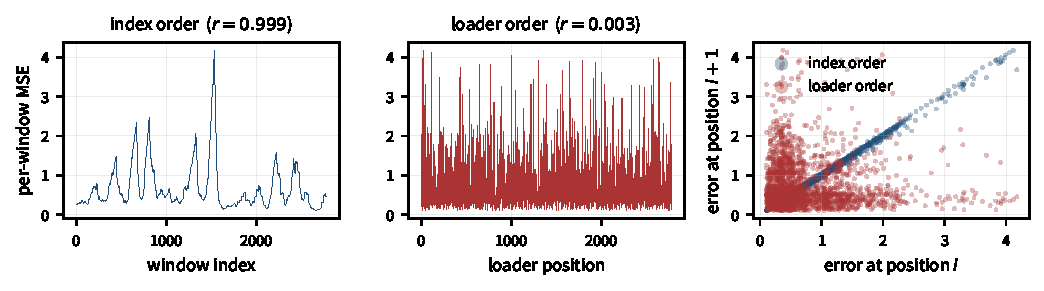
\includegraphics[width=\linewidth]{figs/sequence}
\caption{One real validation error vector in index order (left) and the same
values in loader order (middle), with the lag-1 scatter of both (right). The two
vectors have identical means, quantiles and histograms.}
\label{fig:sequence}
\end{figure}

\subsection{Detector operating characteristics}
\label{sec:res-detect}

Across \NumSequences{} real index-order sequences spanning
\NumWindowsAudited{} evaluation windows (lengths from \NumWindowsMin{} to
\NumWindowsMax{}), the circular serial correlation has median
$\NumRMedianClean{}$ and minimum $\NumRMinClean{}$: window overlap produces
dependence close to the maximum possible, uniformly over datasets, horizons,
backbones and arms. After a uniform permutation of the same sequences the median
falls to $\NumRMedianCorrupt{}$ with maximum $\NumRMaxCorrupt{}$. The standardised
statistic separates the two populations by orders of magnitude
(Figure~\ref{fig:separation}): median $z = \NumZMedianClean{}$ for intact
sequences with a minimum of $\NumZMinClean{}$, against a maximum of
$\NumZMaxCorrupt{}$ over all permuted sequences.

\begin{figure}[t]
\centering
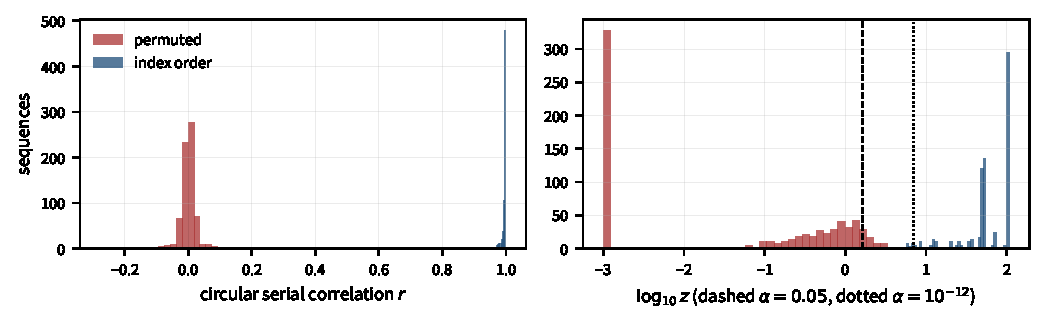
\includegraphics[width=\linewidth]{figs/separation}
\caption{Separation of the AOT statistic on \NumSequences{} real sequences and
their permutations. Left: the raw statistic. Right: the standardised statistic on
a log scale, with the $\alpha = 0.05$ and $\alpha = 10^{-12}$ thresholds.}
\label{fig:separation}
\end{figure}

At $\alpha = 0.05$ the test certifies $\NumCleanCertPct\%$ of intact sequences and
$\NumCorruptCertPct\%$ of permuted ones---the latter is the nominal false
certification rate, as it must be, since permuted sequences are drawn exactly from
the null. Table~\ref{tab:cert} sweeps the level. The row to use in practice is
$\alpha = 10^{-6}$: it separates the two populations \emph{perfectly} on our data,
certifying $\NumCleanCertAlphaSix\%$ of intact sequences and
$\NumCorruptCertAlphaSix\%$ of permuted ones, which is what the margin between
$z_{\min} = \NumZMinClean{}$ on intact sequences and
$z_{\max} = \NumZMaxCorrupt{}$ on permuted ones predicts. Pushing to
$10^{-12}$ costs sensitivity only on the shortest artefacts:
$\NumCleanCertAlphaTwelve\%$ of intact sequences are still certified, and every one
of the \NumCertTwelveMissSeq{} that are not has at most $\NumCertTwelveMissMaxN{}$
windows---AOT's evidence grows with $n$, and an evaluation split of a few dozen
windows simply does not contain twelve orders of magnitude of it. A continuous integration
job can therefore fail the build on order corruption without any realistic risk of
a false alarm, which is the property a diagnostic needs to survive contact with a
busy team.

\begin{table}[t]
\centering
\caption{AOT certification rates as a function of the level, over
\NumSequences{} real sequences and their uniform permutations. Generated from
\texttt{artifacts/certification.csv}.}
\label{tab:cert}
\fitwidth{\begin{tabular}{lrr}
\toprule
$\alpha$ & index-order certified (\%) & permuted certified (\%) \\
\midrule
0.05 & 100.0 & 6.18 \\
0.01 & 100.0 & 1.69 \\
$10^{-3}$ & 100.0 & 0.14 \\
$10^{-6}$ & 100.0 & 0.00 \\
$10^{-12}$ & 97.5 & 0.00 \\
\bottomrule
\end{tabular}}
\end{table}

The normal approximation is not doing hidden work. On \NumCalibSeq{} permuted
sequences, where the null is true by construction, the analytic and Monte-Carlo
$p$-values differ by at most $\NumCalibMaxAbsDiff{}$, and the empirical rejection
rates at $\alpha = 0.05$ are $\NumCalibFprNormal\%$ (analytic) and
$\NumCalibFprPerm\%$ (Monte-Carlo).

\emph{Milder corruptions.} A uniform permutation is the worst case; real defects
can be gentler. Shuffling \emph{batch order} while keeping batches internally
sequential---what a batch-level sampler produces---preserves within-block
dependence, and permuting only a fraction of positions preserves most of it.
Table~\ref{tab:sens} reports detection rates for both families. Block corruption
remains detectable up to blocks of $\NumSensBlockMax{}$ samples
($\NumSensBlockMaxRate\%$ detected), because the reordering still breaks the joins
between blocks; and moving as few as $\NumSensPartialMin\%$ of positions is detected in
$\NumSensPartialMinRate\%$ of sequences. At the other end, a full
permutation is by definition undetectable as a \emph{deviation} from the null---the
$\NumSensPartialFullRate\%$ entry is the nominal rate---which is the point of the
certification framing: we certify the presence of order, not the absence of a
specific corruption.

\begin{table}[t]
\centering
\caption{AOT detection of milder corruptions, over \NumSensSeq{} sequences.
Generated from \texttt{artifacts/aot\_sensitivity.csv}.}
\label{tab:sens}
\fitwidth{\begin{tabular}{llrrr}
\toprule
corruption & parameter & order structure kept (\%) & sequences & AOT flagged (\%) \\
\midrule
block-order shuffle, block size $b$ & 8 & 87.5 & 60 & 0.00 \\
block-order shuffle, block size $b$ & 32 & 96.9 & 60 & 0.00 \\
block-order shuffle, block size $b$ & 128 & 99.2 & 58 & 0.00 \\
block-order shuffle, block size $b$ & 512 & 99.8 & 57 & 0.00 \\
partial shuffle, fraction $f$ moved & 0.05 & 95.0 & 60 & 0.00 \\
partial shuffle, fraction $f$ moved & 0.10 & 90.0 & 60 & 0.00 \\
partial shuffle, fraction $f$ moved & 0.25 & 75.0 & 60 & 1.67 \\
partial shuffle, fraction $f$ moved & 0.50 & 50.0 & 60 & 1.67 \\
partial shuffle, fraction $f$ moved & 1.00 & 0.0 & 60 & 95.00 \\
\bottomrule
\end{tabular}}
\end{table}

\emph{Cross-arm agreement.} On the \NumCatBlocks{} groups of arms evaluated against
a common sample set, CAT gives median $\bar{\rho} = \NumCatRhoMedianClean{}$,
certifying $\NumCatCertCleanPct\%$ of groups; after independent per-arm permutation
the median falls to $\NumCatRhoMedianCorrupt{}$ and $\NumCatCertCorruptPct\%$ are
certified. \NumCatMissGroups{} intact group is not certified, and it is one of the
shortest in the study ($n \le \NumCatMissMaxN{}$ windows, against a minimum of
$\NumCatMinN{}$ over all groups), where four arms simply do not supply enough rank
information; its $\bar{\rho}$ of $\NumCatRhoMinClean{}$ is the minimum over intact
groups. The agreement is not driven by one dominant pair: across all \NumCatPairs{}
individual arm pairs the median Spearman correlation is $\NumCatPairRhoMedian{}$.
Sample difficulty dominating arm identity is a robust empirical regularity, and CAT
converts it into a test.

\subsection{Where each test stops working}
\label{sec:res-battery}

AOT's power comes from window overlap, so we remove the overlap deliberately.
Sub-sampling every $s$-th window reduces the shared fraction of two consecutive
retained windows from $1 - 1/(L+H)$ to $\max(0, 1 - s/(L+H))$, and at large enough
$s$ the retained windows are disjoint. Table~\ref{tab:battery} and
Figure~\ref{fig:battery} trace both tests along that axis. AOT certifies
$\NumBatAotStrideOne\%$ of intact groups at stride $1$ and degrades as overlap
falls; on the \NumBatDisjointRows{} configurations in which the retained windows
are exactly disjoint ($s = \NumBatStrideDisjoint{}$, mean length
$\NumBatNDisjoint{}$) it certifies $\NumBatAotDisjoint\%$. CAT, which never used
serial structure, certifies $\NumBatCatStrideOne\%$ at stride $1$ and
$\NumBatCatDisjoint\%$ on the disjoint grid. Corrupted inputs, pooled over all
\NumBatRows{} configurations of the sweep, are certified at
$\NumBatCorruptAotPct\%$ by AOT and $\NumBatCorruptCatPct\%$ by CAT---the nominal
level, up to the sampling noise of \NumBatGroups{} groups per stride---so the loss
of power at long strides is a loss of \emph{sensitivity}, not a gain in false
alarms. The practical rule follows directly: use AOT when samples overlap, use CAT
whenever two or more arms share a sample set, and treat an artefact that satisfies
neither precondition---a single arm on independent samples---as unauditable after
the fact, which makes the write-side contract mandatory rather than advisable.

\begin{table}[t]
\centering
\caption{The battery against loss of overlap. \emph{Overlap} is the mean shared
fraction of consecutive retained windows; \emph{clean} and \emph{perm.} are
certification rates (\%) on intact and permuted vectors; the permuted columns
estimate the nominal $5\%$ level from \NumBatGroups{} groups per stride, so their
per-row noise is large while the pooled rate quoted in the body is not. Generated from
\texttt{artifacts/battery.csv}.}
\label{tab:battery}
\fitwidth{\begin{tabular}{rrrrrrr}
\toprule
stride & overlap & $n$ & AOT clean & AOT perm. & CAT clean & CAT perm. \\
\midrule
1 & 1.00 & 5250 & 100.0 & 8.7 & 100.0 & 3.8 \\
4 & 0.99 & 1313 & 100.0 & 5.1 & 100.0 & 3.8 \\
16 & 0.95 & 329 & 100.0 & 2.9 & 100.0 & 0.0 \\
64 & 0.78 & 86 & 71.9 & 6.2 & 100.0 & 12.5 \\
192 & 0.41 & 59 & 37.5 & 3.1 & 100.0 & 25.0 \\
\bottomrule
\end{tabular}}
\end{table}

\begin{figure}[t]
\centering
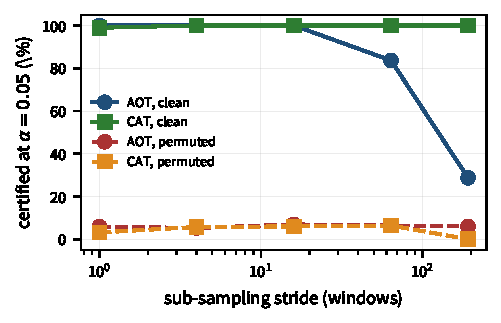
\includegraphics[width=0.62\linewidth]{figs/battery}
\caption{Certification rate against sub-sampling stride. AOT follows the overlap;
CAT does not depend on it. Permuted input is certified only at the nominal level,
at every stride and by both tests.}
\label{fig:battery}
\end{figure}

\subsection{Downstream: a real conclusion changes, and the control does not}
\label{sec:res-downstream}

\emph{T1.} Under the correct join, per-sample loss is genuinely associated with
cheap look-back covariates: across \NumTaskOneCells{} runs the median Spearman
correlation between look-back volatility and loss is
$\NumTaskOneRhoIndexMedian{}$ (mean $\NumTaskOneRhoIndexMean{}$), the best single
covariate reaches $\NumTaskOneRhoBestIndexMedian{}$ in absolute value, and the top
volatility decile is $\NumTaskOneDecileIndexMedian{}\times$ harder than the bottom
decile. The association is significant at $\alpha = 0.05$ in
$\NumTaskOneSigIndexPct\%$ of runs. Under the defect the same numbers become
$\NumTaskOneRhoDefectMedian{}$, $\NumTaskOneRhoBestDefectMedian{}$,
$\NumTaskOneDecileDefectMedian{}\times$ and $\NumTaskOneSigDefectPct\%$: the
effect is gone, the decile contrast is exactly the ratio of two samples from the
same distribution, and a reader would conclude that per-sample difficulty is
unrelated to the obvious drivers of per-sample difficulty. The predictive version
tells the same story---median transfer rank agreement on the untouched test split
falls from $\NumTaskOneTransferIndexMedian{}$ to
$\NumTaskOneTransferDefectMedian{}$, and the purged within-split holdout from
$\NumTaskOneHoldoutIndexMedian{}$ to $\NumTaskOneHoldoutDefectMedian{}$.
Table~\ref{tab:t1} and Figure~\ref{fig:downstream} collect the comparison.

\begin{table}[t]
\centering
\caption{T1 under the three conditions, medians over \NumTaskOneCells{} runs. The
\emph{defect} and \emph{control} columns are two samples from the same
distribution (Proposition~\ref{prop:degeneracy}); the test in the body certifies
that they are, rather than merely failing to distinguish them. Generated from
\texttt{artifacts/t1\_difficulty.csv}.}
\label{tab:t1}
\fitwidth{\begin{tabular}{lrrr}
\toprule
statistic (median over runs) & index order & defect & control \\
\midrule
$\rho$(volatility, error) & 0.219 & -0.000 & 0.001 \\
$\rho$ of the best feature & 0.268 & 0.010 & 0.009 \\
top/bottom decile error ratio & 1.43 & 1.00 & 1.00 \\
transfer rank agreement on test & 0.227 & 0.016 & -0.008 \\
significant association at $\alpha=0.05$ (\%) & 89.3 & 3.9 & 5.3 \\
\bottomrule
\end{tabular}}
\end{table}

\begin{figure}[t]
\centering
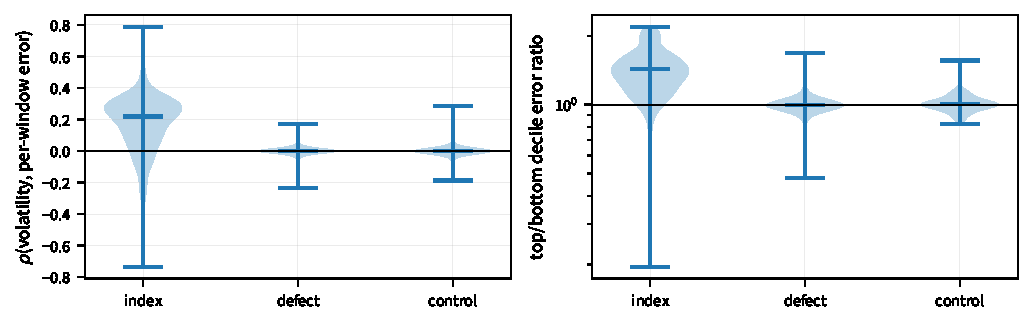
\includegraphics[width=\linewidth]{figs/downstream}
\caption{T1 across \NumTaskOneCells{} runs under the correct join, the defect and
the shuffled-feature control. Left: association between look-back volatility and
per-sample loss. Right: hardness ratio between the top and bottom volatility
decile (log scale; $1$ is no effect).}
\label{fig:downstream}
\end{figure}

The third column of Table~\ref{tab:t1} is the point of the paper. The
shuffled-feature control---the check an author would run to convince a reviewer
that the null in column two is real---lands on the same values as the defect.
We certify this rather than assert it. A two one-sided test of equivalence
\citep{schuirmann1987,lakens2017} on the paired difference between the defect and
the control, with an equivalence margin of $\NumTaskOneTostMargin{}$ Spearman units
(a fifth of the intact effect), gives a mean difference of
$\NumTaskOneTostMeanDiff{}$ with a $95\%$ confidence interval of
$[\NumTaskOneTostCiLow{}, \NumTaskOneTostCiHigh{}]$ and $p = \NumTaskOneTostP{}$:
the two conditions are statistically equivalent, not merely indistinguishable. The
predictive statistic gives the same verdict on the
\NumTaskOneTransferTostN{} runs where transfer rank agreement is defined: a mean
paired difference of $\NumTaskOneTransferTostMeanDiff{}$ with interval
$[\NumTaskOneTransferTostCiLow{}, \NumTaskOneTransferTostCiHigh{}]$ inside a margin
of $\NumTaskOneTransferTostMargin{}$ and $p = \NumTaskOneTransferTostP{}$. Both the
descriptive and the predictive reading of T1 therefore certify that the defect and
the control are the same experiment.

\emph{T2.} The decision analysis behaves the way Proposition~\ref{prop:attenuation}
predicts. Over \NumTaskTwoBlocks{} groups, a per-sample gate trained on the correct
join changes test error by a median of $\NumTaskTwoGainIndexMedian\%$ relative to
the best fixed arm, against a per-sample oracle headroom of
$\NumTaskTwoOracleHeadroomMedian\%$; a positive gain occurs in
$\NumTaskTwoGainIndexPosPct\%$ of groups, and a Wilcoxon signed-rank test of the
gain against zero gives $p = \NumTaskTwoSignTestP{}$. Under the defect the median
gain is $\NumTaskTwoGainDefectMedian\%$ and under the control
$\NumTaskTwoGainControlMedian\%$: both are non-results, as
Proposition~\ref{prop:attenuation} requires.

Here, however, the defect and the control are \emph{not} interchangeable, and
Proposition~\ref{prop:derived} says why. The paired defect-minus-control difference
in gain is $\NumTaskTwoTostMeanDiff{}$ percentage points with interval
$[\NumTaskTwoTostCiLow{}, \NumTaskTwoTostCiHigh{}]$, which excludes zero as well as
the equivalence margin of $\NumTaskTwoTostMargin{}$: the defect is measurably
\emph{worse} than the control, so here the equivalence test correctly declines to
certify equivalence. The label law is where the difference lives. Over the
\NumLabelBlocks{} groups, the per-window best-arm label under the correct join puts
on average $\NumLabelModalIndexPct\%$ of its mass on its modal arm, with mean
entropy $\NumLabelEntropyIndex{}$ bits out of a possible
$\NumLabelEntropyMax{}$; under independent per-arm permutation the modal mass falls
to $\NumLabelModalDefectPct\%$ and the entropy rises to $\NumLabelEntropyDefect{}$
bits, and the share of windows won by the globally best fixed arm falls from
$\NumLabelBestFixedShareIndexPct\%$ to $\NumLabelBestFixedShareDefectPct\%$. The
defect thus flattens the label towards uniform, which is exactly the product-law
statement of Proposition~\ref{prop:derived}. A gate trained on such labels
distributes windows across arms nearly independently of arm quality, and the
realised error drifts towards the uniform-arm baseline, which on this grid costs
$\NumTaskTwoRandomPenaltyMedian\%$ relative to the best fixed arm. The control,
which keeps the label intact and destroys only the features, degenerates to
predicting the modal arm and therefore costs almost nothing. The reading is
uncomfortable and worth stating plainly: for derived-label analyses the standard
negative control is not merely powerless, it understates the damage. We draw a
deliberately limited conclusion from T2---it does \emph{not} establish that
per-sample gating works when the join is correct. Our companion study
\citep{companion2026} examines that question directly and answers it in the negative
for legal feedback delays; the relevant point here is that the two explanations for
a null gate---no learnable signal, or a permuted label column---are not
distinguishable by anything reported in a conventional table, and are
distinguishable in one line by AOT.

\begin{table}[t]
\centering
\caption{T2 under the three conditions, medians over \NumTaskTwoBlocks{} groups.
Unlike T1, the \emph{defect} and \emph{control} columns are not two samples from
the same distribution: the label here is derived from all arms, so
Proposition~\ref{prop:derived} applies and the control is the milder condition.
Generated from \texttt{artifacts/t2\_selection.csv}.}
\label{tab:t2}
\fitwidth{\begin{tabular}{lrrr}
\toprule
statistic (median over blocks) & index order & defect & control \\
\midrule
gain over best fixed arm (\%) & -1.03 & -1.12 & -0.29 \\
per-window oracle headroom (\%) & 8.10 & 8.10 & 8.10 \\
agreement with the per-window oracle & 0.330 & 0.295 & 0.333 \\
blocks with a positive gain (\%) & 25.0 & 8.3 & 15.6 \\
\bottomrule
\end{tabular}}
\end{table}

\subsection{The repair is not free}
\label{sec:res-tax}

The obvious fix is to set the evaluation loader's shuffle flag to \texttt{False}.
It is the right fix, and it is not a silent one. A shuffling loader draws from the
global pseudo-random stream once per epoch; removing those draws shifts every
subsequent consumer of the stream---parameter initialisation of later components,
dropout masks, and the training loader's own shuffling---so the repaired run
follows a different trajectory. Across \NumTaxPairs{} matched pairs that differ in
exactly this flag, the reported test error changes by a median of
$\NumTaxMedianAbs\%$, a ninetieth percentile of $\NumTaxPNinetyAbs\%$ and a
maximum of $\NumTaxMaxAbs\%$; $\NumTaxOverTenthPct\%$ of pairs move by more than a tenth of a
percent, only $\NumTaxIdenticalPct\%$ are numerically identical, the selected
epoch agrees in $\NumTaxSameEpochPct\%$ of pairs, and a Wilcoxon signed-rank test
finds no systematic direction ($p = \NumTaxWilcoxP{}$). Figure~\ref{fig:rngtax}
and Table~\ref{tab:tax} show the distribution.

\begin{table}[t]
\centering
\caption{Cost of the one-line repair: paired change in reported test MSE when the
validation loader stops shuffling. Generated from
\texttt{artifacts/rng\_tax.csv}.}
\label{tab:tax}
\fitwidth{\begin{tabular}{lrrrr}
\toprule
dataset & pairs & median $|\Delta|$ (\%) & max $|\Delta|$ (\%) & same best epoch (\%) \\
\midrule
ETTh1 & 19 & 0.018 & 0.497 & 74 \\
\textbf{all} & 19 & 0.018 & 0.497 & 74 \\
\bottomrule
\end{tabular}}
\end{table}

\begin{figure}[t]
\centering
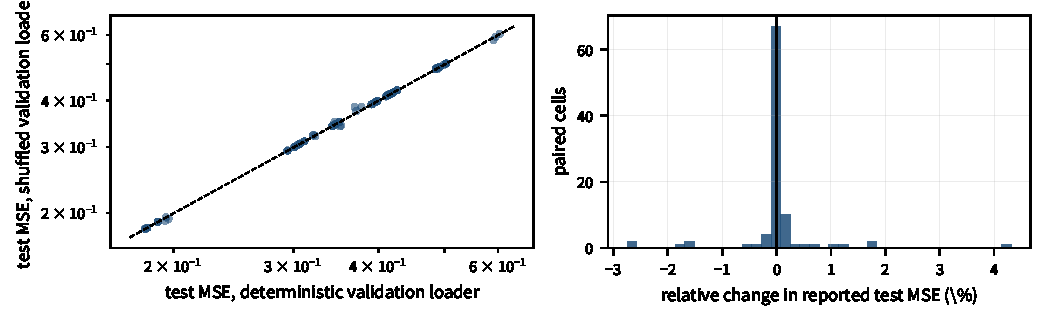
\includegraphics[width=\linewidth]{figs/rngtax}
\caption{The repair changes the run, not just the artefact. Left: paired test MSE
under the two loader settings. Right: distribution of the relative change. The
change has no systematic direction; it is trajectory noise of the size that
tooling-level nondeterminism is known to produce \citep{pham2020,zhuang2022}.}
\label{fig:rngtax}
\end{figure}

The direction of the change is uninteresting and the size is not: it is within
the same order of magnitude as the margins that separate competing methods on
these benchmarks, so it is large enough to move a comparison. The
maintenance consequence is concrete. A team that discovers this fault in a
published pipeline cannot patch the flag and keep the old table---the old table
belongs to a different experiment. They must either re-run everything under the
repaired configuration, or leave the flag alone and adopt the recorder of
Section~\ref{sec:contract}, which fixes the artefact without touching the random
stream. We recommend the second for anything already published, and we note that
this is a good reason for the contract to be a \emph{recording} discipline rather
than a change of loader behaviour.

% =====================================================================
\section{Guidance}
\label{sec:guidance}

The findings compress into a short protocol. We state it as three roles because
the checks that are cheap differ by role.

\paragraph{For authors}
(1) Never write a per-sample artefact without recording the order it is in; the
sidecar of Section~\ref{sec:contract} is the minimum. (2) Load per-sample arrays
through a reader that requires an order, so a positional join cannot be written by
accident. (3) If a per-sample artefact must come from a shuffling loader, record
the sample index alongside the value instead of disabling the shuffle---disabling
it changes the experiment (Section~\ref{sec:res-tax}). (4) Run AOT on every stored
per-sample vector and CAT on every group of arms as part of the test suite, at a
conservative level. (5) When reporting a per-sample \emph{null}, state explicitly
which order check was performed; a shuffled-feature control is not one
(Corollary~\ref{cor:cannot}), and if the analysis selects among several arms the
control is optimistic rather than conservative (Proposition~\ref{prop:derived}).

\paragraph{For reviewers}
When a paper reports a per-sample analysis---difficulty prediction, per-instance
routing, sample-level ablation---the question ``how do you know the two tables are
aligned?'' has, at present, no standard answer, and the answers that sound
convincing (a shape check, a shuffled-feature control, a sensible aggregate) are
all provably uninformative here. Asking for the order check is cheap for an honest
author and diagnostic otherwise. A reported null about per-sample structure
deserves this question more than a reported effect does, because the fault only
produces nulls.

\paragraph{For artefact evaluators}
Badging schemes check that artefacts run and reproduce the reported numbers
\citep{acmbadging,pineau2021,gundersen2018}. Both checks pass under this fault, by
Proposition~\ref{prop:invariance}. A per-sample artefact can be checked further
without the original authors and without a GPU: AOT reads the published vector,
takes $O(n)$ time, and has a calibrated false-alarm rate. We suggest that
artefacts containing per-sample vectors carry order metadata as a condition of the
reusable badge, and note that the check is mechanisable.

% =====================================================================
\section{Threats to validity and limitations}
\label{sec:limits}

\paragraph{Construct}
Our detectors certify the presence of the structure that order induces; they do not
certify alignment. AOT is invariant to circular rotation and nearly invariant to
reversal, and CAT is invariant to a permutation shared by all arms. An off-by-one
write, a reversed sort or a globally shared shuffle therefore pass. We consider
this a limitation of post-hoc auditing in general, not of these statistics in
particular: content-based inference of order can only see structure that the
transformation destroys. The write-side contract is not subject to this limit,
which is why we present it as primary.

\paragraph{Internal}
The observed defect is measured on our own pipeline, in which we deliberately
reproduced the upstream loader policy. The corrupted conditions in T1 and T2 use
permutations drawn the way a defective pipeline draws them---uniformly, and
independently per arm---which matches the observed permutations of our shuffled
runs but is an idealisation of any specific real defect. Our T2 gate is one
reasonable design; a different gate would give different gains under the correct
join. That does not affect the comparison of interest, which is between conditions
holding the gate fixed.

\paragraph{External}
The empirical study is entirely within sliding-window multivariate forecasting on
seven public benchmarks, three backbones and four arms. The formal results
(Propositions~\ref{prop:invariance}--\ref{prop:derived}) require only a
per-sample artefact and a positional join, so they transfer verbatim to
classification, ranking, retrieval or any other per-sample analysis; the
\emph{power} of AOT does not, since it is a function of the serial dependence that
overlapping windows create. Section~\ref{sec:res-battery} quantifies exactly how
that power decays, and CAT is the recommended instrument outside the
sliding-window setting. We have not audited third-party artefacts, and we make no
claim about the prevalence of the fault in the literature; establishing prevalence
would require running the battery over public per-sample artefacts, which is
mechanical, and which we regard as the natural next step rather than as part of
this contribution.

\paragraph{Statistical}
The equivalence tests are paired over runs, and runs within a dataset are not
independent; we therefore report intervals alongside verdicts, and where our
sample cannot certify equivalence at the stated margin we say so rather than
reporting a non-significant difference as an equality. AOT's $p$-values are exact
in the first two moments and asymptotic in the tail; the calibration in
Section~\ref{sec:res-detect} bounds the discrepancy against a Monte-Carlo null at
$\NumCalibMaxAbsDiff{}$, and any application that needs exactness can pay for the
resampling.

% =====================================================================
\section{Related work}
\label{sec:related}

\paragraph{Silent faults in machine-learning software}
Empirical studies of defects in deep-learning programs and frameworks consistently
find that the most damaging class is the one that produces no crash
\citep{zhang2018tf,islam2019}, and \citet{tambon2024} study exactly this class
under the name \emph{silent bugs}, cataloguing framework-level faults that alter
results without raising an error. Our fault is of that kind but at a different
level: it lives in the composition of two individually correct components, and its
observable effect is confined to an artefact's index. To our knowledge the
per-sample order channel has not been analysed, and the interaction with negative
controls has not been noted.

\paragraph{Nondeterminism and variance in training}
That a training run's outcome moves under changes to random state and tooling is
well documented \citep{pham2020,zhuang2022}, and our
Section~\ref{sec:res-tax} is an instance: the flag that causes the fault also
couples the evaluation loader to the training trajectory. The contribution here is
not the observation of variance but its consequence for repair---removing the
shuffle is not a behaviour-preserving refactoring, so an honest fix is a re-run or
a recording discipline, not a patch.

\paragraph{Leakage, reproducibility and evaluation pitfalls}
\citet{kapoor2023} taxonomise leakage as the dominant reproducibility failure in
machine-learning-based science, and reproducibility programmes and badging schemes
formalise what an artefact must contain \citep{pineau2021,gundersen2018,acmbadging}.
Leakage inflates results and is caught by out-of-sample discipline; the fault we
study deflates them and is caught by none of the standard checks, which is why we
treat it as a distinct failure mode rather than a variant. In time series
specifically, evaluation methodology has been scrutinised for split construction
and dependence between folds \citep{bergmeir2012,hyndman2006,makridakis2020m4};
that literature concerns \emph{which} samples are used, whereas our concern is the
identity of a sample once used.

\paragraph{Provenance and workflow systems}
Recording how a derived artefact came about is the subject of a mature literature
\citep{cheney2009,herschel2017}, is operationalised by workflow engines
\citep{ditommaso2017,koster2012} and experiment trackers
\citep{zaharia2018mlflow}, and is codified for scientific data by the FAIR
principles \citep{wilkinson2016}. Our contract is a deliberately minimal
specialisation: for the single property that positional joins depend on, a closed
vocabulary of orders and a reader that fails closed. We see it as an instance of
the general prescription that the ML tooling stack currently omits.

\paragraph{Testing without an oracle}
Metamorphic testing \citep{segura2016,chen2018metamorphic} verifies programs by
checking relations between outputs of related inputs when no oracle is available.
AOT and CAT are statistical relatives: neither knows the correct order, and each
checks a property that the correct order implies---serial dependence for AOT,
cross-arm agreement for CAT. The connection is practically useful, since it places
both tests naturally in a test suite rather than in an analysis notebook.

\paragraph{Negative controls}
Negative controls are a standard device for detecting bias in observational studies
\citep{lipsitch2010}, and their machine-learning analogues---shuffled labels,
shuffled features, random baselines---are used to validate per-sample claims.
Proposition~\ref{prop:degeneracy} identifies a case in which a negative control is
provably uninformative, because the fault it is meant to detect and the control
itself induce the same distribution. We are not aware of a prior statement of this
degeneracy, and we suspect it is not unique to order corruption: any fault that
acts by destroying a pairing will collide with the control that destroys the same
pairing. That suggests a general design rule, which we state as a question for
future work: a negative control is only informative about faults that act
differently from the control.

\paragraph{Time series forecasting and plug-ins}
The empirical carrier of this study is the long-horizon forecasting benchmark
suite \citep{zhou2021informer,wu2021autoformer,zeng2023dlinear,nie2023patchtst,liu2024itransformer}
and the model-agnostic modules attached to it
\citep{kim2022revin,liu2023san,wang2024fredf}, implemented in a common reference
library \citep{tslib,wu2023timesnet}. We use them only as a source of realistic
per-sample artefacts, and we take no position here on the arms' relative merits;
the companion study \citep{companion2026} addresses the selection question.

% =====================================================================
\section{Conclusion}
\label{sec:conclusion}

Per-sample analysis rests on an assumption that is almost never written down: that
two artefacts produced by different parts of a pipeline are in the same order. We
have shown that when the assumption fails, the failure is invisible to every guard
the pipeline applies---the aggregate metric is invariant, the length check is blind
by construction, and, most importantly, the negative control that is supposed to
protect the analysis is \emph{equal in distribution} to the fault it is meant to
detect. A null result about per-sample structure, presented with a well-behaved
shuffled-feature control, is therefore exactly as consistent with a broken join as
with a true null, and nothing in a conventional table can separate the two. The one
class of analyses where the control does behave differently---those whose label is
derived from several independently written vectors---is the class where it is most
misleading, because there it reports a milder failure than the fault produces.

The situation is repairable, cheaply, in two steps. Write-side: attach an order
record to every per-sample artefact and refuse to load one for a positional join
without it. Read-side, for artefacts that already exist: run the two tests we
give. On \NumRuns{} runs the battery certifies $\NumCleanCertPct\%$ of intact
sequences and $\NumCorruptCertPct\%$ of permuted ones at $\alpha = 0.05$, separates
the two populations perfectly at $\alpha = 10^{-6}$, and detects corruptions far
milder than a full permutation. We also found that the obvious one-line repair
silently changes reported numbers by up to $\NumTaxMaxAbs\%$, so a maintainer must
re-run rather than patch---or adopt the recorder, which fixes the artefact and
leaves the run alone.

Two directions follow. The first is mechanical and, we think, worth doing: run the
battery over the per-sample artefacts that accompany published papers and measure
how often the fault is present in the wild. The second is conceptual. Our
degeneracy result is an instance of a pattern---a control that destroys the same
structure as the fault cannot see the fault---and we expect other instances to
exist wherever a validation device and a failure mode act through the same
mechanism. Cataloguing them would tell us which of the checks we currently trust
are load-bearing.

% =====================================================================
\printcredits

\section*{Declaration of competing interest}
The authors declare that they have no known competing financial interests or
personal relationships that could have appeared to influence the work reported in
this paper.

\section*{Funding}
This research did not receive any specific grant from funding agencies in the
public, commercial, or not-for-profit sectors.

\section*{Declaration of generative AI and AI-assisted technologies in the
writing process}
During the preparation of this work the authors used a large language model to
assist with copy-editing, LaTeX formatting and the drafting of analysis and
plotting scripts. All experimental design, statistical decisions, numerical
results and scientific conclusions were produced and verified by the authors, who
take full responsibility for the content of the publication.

\section*{Relation to other work by the authors}
This study and the companion manuscript \citep{companion2026} share an
experimental infrastructure and a research programme but address disjoint
questions and report disjoint results: the companion asks whether per-window
plug-in selection is learnable under legal feedback delay, and this paper asks
whether a per-sample artefact is in the order its consumer assumes. Neither
manuscript's claims depend on the other's; the overlap is disclosed here so that
editors and reviewers can assess it directly.

\section*{Data availability}
All datasets used in this study are public standard benchmarks (ETT, Weather,
Exchange-Rate, ILI) and are not redistributed here; the release includes the
download script and the checksums we verified. Everything required to recompute
every number, table and figure in this manuscript is released at
\url{https://github.com/oscarliu2019/order-provenance-audit}: the experiment
configuration; the per-run table for all \NumRuns{} runs; the per-sample audit
outputs (AOT sequence statistics, calibration, sensitivity, certification sweep,
cross-arm agreement, the battery); the per-sample feature tables; the T1 and T2
outputs and the equivalence tests; the paired repair-cost table; the reference
implementation of the order contract and of both tests; the test suite covering the
propositions as executable statements; and the generators for
\texttt{paper/numbers.tex}, all tables and all figures. A verification script,
\texttt{tools/verify\_paper\_numbers.py}, re-derives every quantitative claim in
this manuscript from those artefacts and fails on any mismatch, printing the claim
identifier, the printed value and the recomputed value.

\bibliographystyle{elsarticle-num-names}
\bibliography{refs}

\end{document}
